%LaTeX template : http://systbio.org/files/SB_LaTeX_Template_txt_extension.txt
%Author instructions: http://www.oxfordjournals.org/our_journals/sysbio/for_authors/ms_preparation.html


\documentclass[12pt,letterpaper]{article}

%Packages
\usepackage{fixltx2e}
\usepackage{textcomp}
\usepackage{fullpage}
\usepackage{natbib}
\usepackage{float}
\usepackage{latexsym}
\usepackage{hyperref}
\usepackage{url}
\usepackage{hyperref}
\usepackage{epsfig}
\usepackage{graphicx}
\usepackage{amssymb}
\usepackage{amsmath}
\usepackage{bm}
\usepackage{array}
\usepackage[version=3]{mhchem}
\usepackage{ifthen}
\usepackage{caption}
\usepackage{hyperref}
\usepackage{amsthm}
\usepackage{amstext}
\usepackage{enumerate}
\usepackage[osf]{mathpazo}
\pagenumbering{arabic}

%Pagination style and stuff
\linespread{1.66}
\raggedright
\setlength{\parindent}{0.5in}
\setcounter{secnumdepth}{0} 
\renewcommand{\section}[1]{%
\bigskip
\begin{center}
\begin{Large}
\normalfont\scshape #1
\medskip
\end{Large}
\end{center}}
\renewcommand{\subsection}[1]{%
\bigskip
\begin{center}
\begin{large}
\normalfont\itshape #1
\end{large}
\end{center}}
\renewcommand{\subsubsection}[1]{%
\vspace{2ex}
\noindent
\textit{#1.}---}
\renewcommand{\tableofcontents}{}
\bibpunct{(}{)}{;}{a}{}{,}

%---------------------------------------------
%
%       START
%
%---------------------------------------------

\begin{document}
%\modulolinenumbers[1]     % Line numbering on every line

%Running head
\begin{flushright}
Version dated: \today
\end{flushright}
\bigskip
\noindent RH: Missing data and topology in total evidence approach

\bigskip
\medskip
\begin{center}

\noindent{\Large \bf Effect of missing data on topological inference using a total evidence approach}
% TG: Or "Effect of missing data and inference method on topology when using a total evidence approach"
% TG: Or any other suggestions?

\bigskip

%Authors
\noindent {\normalsize \sc Thomas Guillerme$^1$$^,$$^2$, and Natalie Cooper$^1$$^,$$^2$}\\
\noindent {\small \it 
$^1$School of Natural Sciences, Trinity College Dublin, Dublin 2, Ireland;\\
$^2$Trinity Centre for Biodiversity Research, Trinity College Dublin, Dublin 2, Ireland;}\\
\end{center}
\medskip
\noindent{\bf Corresponding author:} Thomas Guillerme, School of Natural Sciences, Trinity College Dublin, Dublin 2, Ireland; E-mail: guillert@tcd.ie; Fax: +353 1 6778094; Tel: +353 1 896 2571.\\
\vspace{1in}

%---------------------------------------------
%
%       ABSTRACT
%
%---------------------------------------------

\newpage
\begin{abstract}
Living species represent a marginal part of all species that have ever lived. Ignoring fossil taxa may lead to misinterpretation of macroevolutionary patterns and processes such as trends in species richness, biogeographical history or paleoecology. This fact has led to an increasing consensus among scientists that both living and fossil taxa must be included in macroevolutionary studies. One approach called Total Evidence, uses molecular data from living taxa and morphological data from both living and fossil taxa to infer phylogenies with both living and fossil taxa at the tips. Although the Total Evidence approach seems very promising, it requires a lot of data and is therefore likely to suffer from missing data issues which may affect its ability to infer correct phylogenies.

In this study we assess the effect of missing data on tree topologies inferred from Total Evidence matrices. Using simulations we investigate three major factors that directly affect the completeness of the morphological part of the matrix: (1) the proportion of living taxa with no morphological data, (2) the amount of missing data in the fossil record, and (3) the overall number of morphological characters in the matrix. 

We find that, when using a clade conservative metric such as Robinson-Foulds distance, Bayesian consensus trees recovers the right topology better than Maximum Likelihood or than a subset of Bayesian posterior tree distributions and this regardless of the amount of missing data (minimal tree similarity of 0.69 in the worst scenario). Regarding the data, good topological recovery is not related to the amount of missing data \textit{per se} but to the amount of data overlap. The two factors that influences the most this data overlap are the parameters 1 (proportion of coded living taxa) and 3 (number of morphological characters).

%Probably needs to be deeeply rewritten, as said last time to Kev quoting Stuart Pim, people only read the abstract.
% NC: Yep, for now I'll leave this

\end{abstract}

\noindent (Keywords: missing data, Total Evidence, Bayesian, Maximum Likelihood, topology)\\

\vspace{1.5in}

\newpage 

%---------------------------------------------
%
%       INTRODUCTION
%
%---------------------------------------------

\section{Introduction}

Although most species that have ever lived are now extinct \citep{novacek1992ext,raup1993extinction}, the majority of macroevolutionary studies focus solely on living species \citep[e.g.][]{meredithimpacts2011,jetzthe2012}. Ignoring fossil taxa may lead to misinterpretation of macroevolutionary patterns and processes such as the timing of diversification events \citep[e.g.][]{pyrondivergence2011}, relationships among lineages \citep[e.g.][]{manosphylogeny2007} or niche occupancy \citep[e.g.][]{pearmanniche2008}. This has led to increasing consensus among evolutionary biologists that fossil taxa should be included in macroevolutionary studies \citep{jacksonwhat2006,quentaldiversity2010,dietlconservation2011,slaterunifying2013,fritzdiversity2013}. However, to do this we need to be able to place living and fossil taxa into the same phylogenies; a task that remains difficult despite recent methodological developments \citep[e.g.][]{pyrondivergence2011,ronquista2012,BEASTmaster}. %Or is it cheap to cite unpublished work (Nick's proto package) in the intro?
% NC: Check Syst Biols policies, but I think it's fine as it's an available package so it'd be like citing something from GitHub. You could ask Nick before publication if there's a different citation he'd prefer you to use.

Up to now, three main approaches have been used to place both living and fossil taxa into phylogenies. These approaches differ mainly in whether they treat fossil taxa as tips or as nodes in the phylogeny, and in which part of the available fossil data is used (i.e. the age of the fossil only or both its age and morphology). Classical cladistic methods use matrices containing morphological data from both living and fossil taxa and treat each taxon as a tip in the phylogeny. Relationships among the taxa are then inferred using optimality criteria such as maximum parsimony \citep{simpson1945}. This approach is commonly used by paleontologists but it ignores the additional molecular data available from living species and does not allow use of probabilistic methods for dealing with phylogenetic uncertainty. Neontologists, on the other hand, more commonly use probabilistic approaches (e.g. Maximum Likelihood or Bayesian methods) based on matrices containing only molecular data from living species. Because fossil taxa do not usually have available DNA, fossils are used as nodes rather than tips in these phylogenies and their occurrence dates are used to time calibrate phylogenies \citep{zuckerkandl1965}. There have been great improvements in the theory and application of these two approaches \citep[e.g.][]{bapsta2013,stadlerdating2013,heaththe2013} as well as much debate about the "best" approach to use \citep[e.g.][]{spencerefficacy2013,wrightbayesian2014}. However neither approach uses all the available data.

A final approach, known as the Total Evidence method, uses matrices containing molecular data from living taxa and morphological data from both living and fossil taxa \citep{eernissetaxonomic1993}. This approach treats every taxon as a tip in the phylogeny, uses the occurrence age of the fossils to time calibrate the phylogeny (known as tip-dating; \citealt{ronquista2012}), and allows the use of probabilistic methods for estimating phylogenetic uncertainty \citep{ronquista2012}. Total Evidence methods have been successfully applied to empirical data \citep[e.g.][]{pyrondivergence2011,ronquista2012,schragocombining2013,slaterphylogenetic2013,beckancient2014}, and are becoming an increasingly popular way of adding fossil taxa to phylogenies. However, although the Total Evidence approach seems very promising, there is one big drawback in using this approach: it requires a lot of data that can be difficult (or impossible) to collect. The morphological data for living taxa are rarely collected when molecular data are available (e.g. \citealt{O'Leary08022013} \textit{vs.} \citealt{meredithimpacts2011}), and for fossil taxa, data can only be collected from features preserved in the fossil record (for example, in vertebrates, the hardest parts of the skeleton are more often preserved than soft parts; \citealt{sansomfossilization2013}). Therefore Total Evidence matrices are likely to contain a lot of missing data that may affect the method's ability to infer correct topologies, branch lengths and support values \citep{salamin2003}. 

%TG: I completely removed this paragraph
%The effect of missing data on phylogenetic inferences has been widely studied \citep{wiensmissing2003,wiensmissing2006,wiensmissing2008,lemmonthe2009,rouresite-specific2011,sansomfossilization2013,pattinsonphylogeny2014,sansombias2014}. Missing molecular data has been seen by some authors as an issue because it can, in some parts of the tree, decrease phylogenetic signal (i.e. the evolutionary information contained within the matrix allowing the inference of topology and branch lengths), especially when using large matrices \citep{lemmonthe2009}. However, this may not be a major issue because phylogenetic signal is easily increased by: (i) including a "modest" number (\texttildelow % NC: This symbol doesn't show up on my PDF. Check.
%50) of highly-covered genes (i.e. a number of genes that are available for all taxa; \citealt{rouresite-specific2011}); (ii) adding a greater number of taxa (especially slowly-evolving taxa or taxa close to the outgroup; \citealt{rouresite-specific2011}); and (iii) choosing more appropriate models of sequence evolution \citep{wiensmissing2006,wiensmissing2008,rouresite-specific2011}. Similarly, missing morphological data might be seen as either a major or minor issue for accurately inferring phylogenies depending on the study in question \citep{wiensmissing2003,sansomfossilization2013,pattinsonphylogeny2014}. Because soft-tissue characters are rarely preserved in the fossil record, missing data is mainly found in these characters, and is therefore not randomly distributed which can lead to biased placement of fossil taxa in phylogenies (e.g. \citealt{sansomfossilization2013}, but see \citealt{pattinsonphylogeny2014}). However, the phylogenetic signal is not related to the amount of missing data \textit{per se} but to the number of informative characters for each taxon, therefore missing data is less of an issue than the number of shared informative characters \citep{kearneyfragmentary2002,wiensmissing2003,pattinsonphylogeny2014}.
% NC: I'm a little dubious of what this paragraph is trying to get at in places. We should discuss at some point. TG: my idea was to do the "literature-review" part of the intro: missing data is already widely studied (answer to the comment: "hun... We already knew that") but it has never been studied in TEM framework. And that's kind of the point we're getting toward with our work: we don't really care about the effect of missing data per se (i.e. what's the threshold where it starts fucking up the phylogeny) but more the fact that Bayesian fails.
% NC: OK fair enough. I think though if this is too long we can probably cut this paragraph and put a bit of it into the paragraph below.

Although missing data does not appear be a major problem in molecular and morphological matrices separately (as long as enough data overlaps in each case) \citep{wiensmissing2003,wiensmissing2006,wiensmissing2008,rouresite-specific2011,pattinsonphylogeny2014}, it may become more of an issue in Total Evidence matrices containing both molecular and morphological data for living and fossil taxa. This may be particularly problematic as fossil taxa (generally) do not have molecular data, resulting in a large section of missing data in Total Evidence matrices. Until now, no attempt has been made to study the impact of this issue on phylogenetic inference using Total Evidence methods.

In this study, we focus on the effect of missing data on our ability to recover a "best" tree's topology because it is a crucial aspect of a phylogeny in many macroevolutionary studies, for example when trying to elucidate the evolutionary relationships among species \citep[e.g.][]{meredithimpacts2011,jetzthe2012}, or for studying evolutionary transitions \citep[e.g.][]{}. %CITE-check Lloyd and Friedman or birdy stuff
Although branch length estimation is also important (namely for timing extinction and/or speciation events - e.g. \citealt{ronquista2012}), we do not consider branch lengths in this study. This is partially due to difficulties with simulating branch lengths and topology simultaneously,
but also because previous studies have already empirically assessed the effect of the Total Evidence method on branch length variation but with a fixed topology approach \citep{ronquista2012,schragocombining2013,slaterphylogenetic2013,beckancient2014}.
Thus understanding the sensitivity of topology to missing data is important for assessing the accuracy of tree estimation in the Total Evidence framework. To our knowledge, this question has never been formally assessed.

Here we use a simulation approach to assess the effect of missing data on tree topologies inferred from Total Evidence matrices. Since the molecular part of a Total Evidence matrix acts like a "classical" molecular matrix containing only the living taxa \citep{ronquista2012}, the effect of missing data on such matrices is well known \citep{wiensmissing2006,wiensmissing2008,rouresite-specific2011}. Therefore, we focus only on missing data in the morphological part of the matrix. We investigate three major parameters that directly affect the completeness of the morphological part of the matrix: (i) the proportion of living taxa with no morphological data; (ii) the proportion of missing data in the fossil taxa; and (iii) the proportion of missing morphological characters for both living and fossil taxa in the matrix. We remove data from a Total Evidence matrix by changing the values of these three parameters and then assess how this affects the topology of trees inferred using Maximum Likelihood and Bayesian methods. We chose these parameters because they reflect empirical biases in data availability. The advent of molecular phylogenetics means that morphological data for living species is rarely collected, and few people have the skills to identify characters needed for detailed phylogenetic analysis. Missing data in fossil taxa is very common due to preservation biases \citep{sansomfossilization2013}, and the overall number of characters depends on the effort of the people identifying them \citep[e.g.][]{O'Leary08022013}. We find that the ability of Total Evidence methods to recover the "best" tree's topology is increased when using Bayesian methods. Also minimizing the proportion of living taxa with no morphological data and the proportion of missing morphological characters improves the ability of Total Evidence methods to recover the "best" tree's topology more so than minimizing the proportion of missing data in the fossil record.

%---------------------------------------------
%
%       METHODS
%
%---------------------------------------------
 
\newpage

\section{Methods}
To explore how missing data in the morphological sections of Total Evidence matrices influences tree topology, we used the following protocol (note that we explain each step in detail below this general outline; Fig.~\ref{Fig_Outline}).
\begin{enumerate}
\item{Generating the matrix:} \label{step:generate_matrix} \\
We randomly generated a birth-death tree (hereafter called the "true" tree) and used it to infer a matrix containing both molecular and morphological data for living and fossil taxa (hereafter called the "complete" matrix).
\item{Removing data:} \label{step:remove_data} \\
We removed data from the morphological part of the "complete" matrix to simulate the effects of missing data by modifying three parameters (i) the proportion of living taxa with no morphological data ($M_{L}$), (ii) the proportion of missing data in the fossil taxa ($M_{F}$) and (iii) the proportion of missing morphological characters ($M_{C}$). The resulting 125 matrices are called hereafter "missing-data" matrices.
\item{Inferring phylogenies:} \label{step:build_phylo} \\
We inferred phylogenetic trees from the "complete" matrix and from the 125 "missing-data" matrices resulting in one tree generated from a matrix containing no missing data (hereafter called the "best" tree) and 125 trees inferred from the matrices with missing morphological data (hereafter called the "missing-data" trees). Phylogenies were inferred via both Maximum Likelihood and Bayesian approaches.
\item{Comparing topologies:} \label{step:compare_topo} \\
We compared the "best" tree to the "missing-data" trees to assess the influence of each parameter ($M_{L}$, $M_{F}$, $M_{C}$) and their interactions on the topologies of our phylogenies
\end{enumerate}
We repeated these four steps 50 times to account for variation in our random parameters in the simulations.

\begin{figure}
\centering
    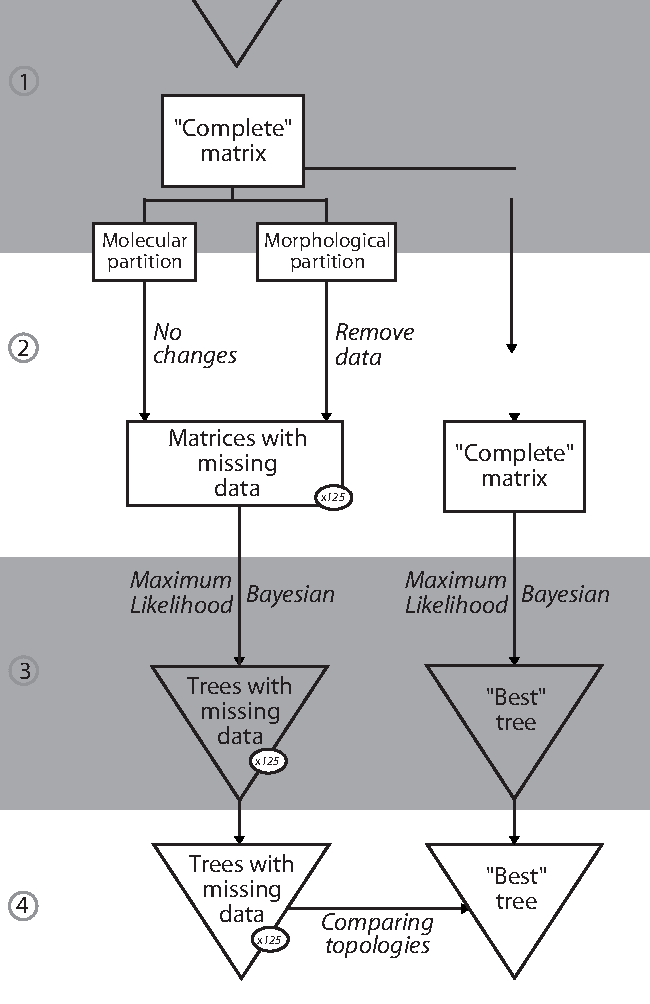
\includegraphics[keepaspectratio=true]{Figures/In_main/Simulations_outline-BW.pdf}
\caption{Protocol outline.
(1) We randomly generated a birth-death tree (the "true" tree) and used it to infer a matrix with no missing data (the "complete" matrix).
(2) We removed data from the morphological part of the "complete" matrix resulting in 125 "missing-data" matrices.
(3) We built phylogenetic trees from each matrix using both Maximum Likelihood and Bayesian methods.
(4) We compared the "missing-data" trees to the "best" tree.
We repeated these four steps 50 times.}
\label{Fig_Outline}
\end{figure}
% NC: Can you centre these around the boxes? and make the comparing topologies arrow touch the two triangles? I'll show you what I mean. 
% NC: Also check the figure is in a format and of correct quality for Syst Biol.

%---------------------------------------------
%       1-Generating the matrix
%---------------------------------------------

\subsection{1-Generating the matrix}
First we randomly generated a "true" tree of 50 taxa in R v. 3.0.2 \citep{R302} using the package diversitree v. 0.9-6 \citep{fitzjohndiversitree2012}. We generated the tree using a birth death process by sampling speciation ($\lambda$) and extinction ($\mu$) rates from a uniform distribution but maintaining $\lambda$ $>$ $\mu$ \citep{paradistime-dependent2011}. We implemented a rejection sampling algorithm to select only trees with 25 living and 25 fossil taxa to ensure that we had enough taxa of each type for our missing data simulations to work. We then added an outgroup to the tree, using the mean branch length of the tree to separate the outgroup from the rest of the taxa, and with the branch length leading to the outgroup set as the sum of the mean branch length and the longest root-to-tip length of the tree.

Next, we generated a molecular and a morphological matrix from the "true" tree. The molecular matrix was inferred from the "true" tree using the R package phyclust v. 0.1-14 \citep{chen2011}. The matrix contained 1000 character sites for 51 taxa and was generated using the seqgen algorithm \citep{ranbaut1997seqgen} and using the HKY model \citep{HKY85} with random base frequencies and transition/transversion rate of two \citep{douadycomparison2003}. The substitution rates were distributed following a gamma distribution with an alpha ($\alpha$) shape of 0.5 \citep{yangamong-site1996}. We chose a low value of $\alpha$ to reduce the number of sites with high substitution rates, thus avoiding too much homoplasy and a decrease in phylogenetic signal. We selected the parameters above to generate data with no special assumption about how the characters evolved, and to reduce the computational time required if these parameters were estimated rather than defined in the tree building part of the analysis (even with the parameters defined, total computational time for the whole analysis was around 150 CPU years). All the molecular information for fossil taxa was replaced by missing data ("?").

We inferred the morphological matrix using the R package ape v. 3.0-11 \citep{paradisape:2004} to generate a matrix of 100 character sites for 51 taxa. We assigned the number of character states (either two or three) for each morphological character by sampling with a probability of 0.85 for two states characters and 0.15 for three state characters. These probabilities were selected using the overall distribution of character states extracted from 100 published empirical morphological matrices (See \hyperref[SupplementaryMaterial]{Supplementary Material Section 1}). We then ran an independent discrete character simulation for each character using the "true" tree with the character's randomly selected number of states (two or three) and assuming an equal rate of change (i.e. evolutionary rate) from one character state to another \citep{Pagel22011994}. This method allows us to have only two parameters for each character: the number of states and the evolutionary rate. For each character, the evolutionary rate was sampled from a gamma distribution with $\alpha$ = 0.5. We used low evolutionary rate parameters to avoid homoplasy in the morphological part of the matrix and create a clear phylogenetic signal \citep{wagner2000,davalosintegrating2014,wrightbayesian2014}.

Finally, we combined the morphological and molecular matrices obtained from the "true" tree. Hereafter we call this the "complete" matrix, i.e. the matrix with no missing data except for the molecular data of the fossil taxa.

%---------------------------------------------
%       2-Removing data
%---------------------------------------------

\subsection{2-Removing data}
\label{Removing_data}
We modified the "complete" matrix to get matrices with missing data by randomly replacing data with "?" in the morphological part of the matrices according to the following parameters:

\begin{enumerate}
\item{$M_{L}$, the proportion of living taxa with no morphological data: 0\%, 10\%, 25\%, 50\% or 75\%.}
This parameter illustrates the number of living taxa that are present in the molecular part of the matrix but not in the morphological part. This reflects the fact that detailed morphological data for living species are scarce.
\item{$M_{F}$, the proportion of missing data in the fossil taxa: 0\%, 10\%, 25\%, 50\% or 75\%.}
This parameter illustrates the quality of the fossil record. 
\item{$M_{C}$, the proportion of missing morphological characters for both living and fossil taxa: 0\%, 10\%, 25\%, 50\% or 75\%. }
This parameter illustrates the number of available morphological characters for both living and fossil taxa.
\end{enumerate}

In practice, each parameter represents a different way of removing data from the matrix: $M_{L}$ removes rows from the living taxa's data; $M_{F}$ removes cells from the fossil taxa's data; and $M_{C}$ removes columns across both living and fossil taxa's data. Note that $M_{L}$ and $M_{F}$ differ not only because of the region of the matrix affected: for $M_{L}$ all the morphological data of a percentage of living taxa is removed, whereas for $M_{F}$ a percentage of the data is removed at random from across the whole of the morphological matrix for fossil taxa.

We created matrices using all parameter combinations resulting in 125 ($5^3$) matrices. Note that one of these combinations has no missing data so is equivalent to the "complete" matrix, thus we have one effectively complete matrix in our 125 "missing-data" matrices. Because some parameter combinations introduce a lot of missing data (e.g. $M_L$=75\%, $M_F$=75\% and $M_C$=75\%), some matrices contained fossil taxa without any data at all. When this occurred we repeated the random deletion of characters until each taxon had at least 5\% data across the whole morphological part of the matrix.

%---------------------------------------------
%       3-Building phylogenies
%---------------------------------------------

\subsection{3-Building phylogenies}
From the resulting matrices we generated two types of trees: the "best" tree inferred from the "complete" matrix and the "missing-data" trees inferred from the 125 matrices with various amounts of missing data. The "true" tree was used to generate the "complete" matrix and reflects the "true" evolutionary history in our simulations. The "best" tree, on the other hand, is the best tree we can build using state-of-the-art phylogenetic methods. In real world situations, the "true" tree is never available to us because we cannot know the true evolutionary history of a clade (except in very rare circumstances, e.g. \citealt{rozen2005}). Therefore, here we focus on comparing the trees inferred from the matrices with missing data to the "best" tree, rather than the "true" tree, as the "best" tree is generally what we have to work with.

\subsubsection{Maximum Likelihood}
The "best" tree and the "missing-data" trees were inferred using RAxML v. 8.0.20 \citep{Stamatakis21012014}. For the molecular data, we used the GTR + $\Gamma_4$ model (\citealt{tavare1986}; default GTRGAMMA in RAxML v. 8.0.20; \citealt{Stamatakis21012014}).% as a generalization of the HKY + $\Gamma_4$ model \citep{HKY85}. The GTR model can be seen as a generalization of the HKY model (the two parameters from the HKY model are implicitly included in the six from GTR model - \citealt{stamatakisa2008}).
For the morphological data, we used the implemented Markov \textit{k} state model \citep{lewisa2001} %which is a generalization of the JC69 model \citep{jc69} with \textit{k} $\geq$ 2
 assuming an equal state frequency and a unique overall substitution rate ($\mu$) following a gamma distribution of the rate variation with four distinct categories (M\textit{k} + $\Gamma_4$; -K MK option in RAxML v. 8.0.20; \citealt{Stamatakis21012014}).

To measure the phylogenetic signal of our simulations, we first ran a fast bootstrap analysis (Lazy Sub-tree Rearrangement) with 500 replicates on the "complete" matrix. We removed all the simulations with a median bootstrap support lower than 50 as a proxy for weak phylogenetic signal \citep{zanderminimal2004}. We repeated this selection until we obtained 50 sets of simulations (i.e. 50 "complete" and 50 x 125 "missing-data" matrices) with a relative good phylogenetic signal (median bootstrap $>$ 50). On these selected simulations, we used the fast bootstrap algorithm and performed 1000 bootstraps for each tree inference to assess topological support \citep{pattengale2010many}.
%The bootstrap algorithm used in RAxML is the Lazy Sub-tree Rearrangement (LSR) which consists of pruning one sub-tree from the tree and subsequently reinserting it to all neighbouring branches \citep{stamatakisa2008}. Sub-tree Pruning and Reinserting methods (SPR) have been demonstrated to be better than other methods (e.g. Nearest Neighbouring Interchange - NNI) for recovering good bootstrap values \citep{salamin2003}.
Using these parameters took \texttildelow 8 CPU years to build 50 sets of 125 bootstrapped Maximum Likelihood trees (2.30GHz clock speed nodes).

\subsubsection{Bayesian}
The "best" tree and the "missing-data" trees were inferred using MrBayes v. 3.2.1 \citep{Ronquist2012mrbayes}. We partitioned the data to treat the molecular part as a non-codon DNA partition and the morphological part as a multi-state morphological partition. The molecular evolutionary history was inferred using the HKY model with a transition/transversion ratio of two \citep{douadycomparison2003} and a gamma distribution for the rate variation with four distinct categories (HKY + $\Gamma_4$). For the morphological data, we used the Markov \textit{k} state model \citep{lewisa2001}, with equal state frequency and a unique overall substitution rate ($\mu$) with four distinct rates categories (M\textit{k} + $\Gamma_4$). We chose these models to be consistent with the parameters used to generate the "complete" matrix.

Each Bayesian tree was estimated using two runs of four chains each for a maximum of 5$\times$$10^7$ generations. We used the following priors for each tree: (i) the "true" tree’s topology as a starting tree (with a starting value for each branch length of one), (ii) an exponential prior on the shape of the gamma distribution of $\alpha$ = 0.5 for both partitions, and (iii) a transition/transversion ratio prior of two sampled from a strong beta distribution ($\beta$(80,40)). We used these priors to speed up the Bayesian estimation process. These priors biased the way the Bayesian process calculated branch lengths by giving non-random starting points and boundaries for parameter estimation however, here we are focusing on the effect of missing data on tree topology and not branch lengths. Even using these priors, it took \texttildelow 140 CPU years to build 50 sets of 125 Bayesian trees (2.30GHz clock speed nodes). The detailed MrBayes parameters are available in the \hyperref[SupplementaryMaterial]{Supplementary Material S1}.

We used the average standard deviation of split frequencies (ASDS) as a proxy to estimate the convergence of the chains and used a stop rule when the ASDS went below 0.01 \citep{Ronquist2012mrbayes}. The effective sample size (ESS) was also checked on a random sub-sample of runs in each simulation to ensure that ESS $>>$ 200 \citep{drummond2006ess}. Finally we built the Bayesian consensus tree from the combined chains excluding the 25\% first iterations (burn-in) with a strict majority rule \citep{Ronquist2012mrbayes}.
%---------------------------------------------
%       4-Comparing Topologies
%---------------------------------------------

\subsection{4-Comparing topologies}
We compared the topology of the "missing-data" trees to the "best" tree to measure the effect of the three parameters $M_{L}$, $M_{F}$ and $M_{C}$ on tree topology. We used the Robinson-Foulds distance \citep{RF1981} to assess the amount of conserved clade positions and the Triplets distance \citep{dobson1975triplets} to assess the amount of wildcard taxa  (i.e. taxa that frequently change position in different trees - \citealt{kearneyfragmentary2002}). We normalised both metrics using the Normalized Tree Similarity index \citep{Bogdanowicz2012} to generalize our results for any \textit{n} number of taxa. These metrics are described in detail below.

\subsubsection{Robinson-Foulds distance}
The Robinson-Foulds distance \citep{RF1981}, or "path difference", measures the number of shared clades across two trees. The metric reflects the distance between the distributions of tips among clades in the two trees (\citealt{RF1981}; see \hyperref[SupplementaryMaterial]{Supplementary Material S2} for calculation details). This metric is bounded between one, when the two trees are identical, and $n-2$ (for two trees with $n$ taxa) when there is no shared clade in the two trees. This metric is sensitive to minor changes in clade conservation: if the trees are composed of two clades of three taxa (\textit{(((a,b),c),((d,e),f))}), the swapping of any two taxa will lead to a maximal score of the Robinson-Foulds distance indicating poor tree similarity. We normalised this metric by % NC: DETAILS 
\citep{Bogdanowicz2012}. This allows us to compare the metric for any number of taxa by scaling it with the expected value of the metric when comparing two random trees (see \hyperref[SupplementaryMaterial]{Supplementary Material S2} for the calculation details). Therefore, when the Normalised Robinson-Foulds distance between two trees is equal to one, the trees are identical; if the distance is equal to zero, the trees are no more different than expected by chance; finally if the distance is less than zero, the trees are more different than expected by chance.

\subsubsection{Triplets distance}
The Triplets distance \citep{dobson1975triplets} measures the number of sub-trees made up of three taxa that differ between two trees (\citealt{critchlowthe1996}; see \hyperref[SupplementaryMaterial]{Supplementary Material S2} for calculation details). This metric measures the position of each taxon and clade in relation to its closest neighbours. It is bounded between 0 when the two trees are identical and $\binom{n}{4}$ (for two trees with $n$ taxa) when there is no shared taxa/clade position in the two trees. Therefore this metric sensitive to the conservation of wildcard taxa. We normalised this metric in the same way as for the Robinson-Foulds distance resulting in the Normalised Triplets distance.

\subsubsection{Paired trees comparisons}
\label{tree_comparisons}
For the Maximum Likelihood and Bayesian consensus trees we performed pairwise comparisons between the "best" tree and each "missing-data" tree using both the Normalised Robinson-Foulds and Normalised Triplets metrics with the TreeCmp java script \citep{Bogdanowicz2012} resulting each time in 125 Normalised Robison-Foulds distances and 125 Normalised Triplets distance. %For each metric, we then normalized the value using the Normalized Tree Similarity scaled by the mean value of 1000 pairwise random tree comparisons for the metric in question and n = 51 taxa (see \hyperref[SupplementaryMaterial]{Supplementary Material Section 2}).
%We compared each "missing-data" tree with the "best" tree for each of our 50 simulation runs resulting in 50 comparisons for each "missing-data" tree. We calculated the mode and the 50\% and 95\% confidence intervals from the resulting distribution using the hdrcde R package v3.1 \citep{hdrcde}.
Also, to take into account the uncertainty of tree inference in both methods cited above, instead of using the single Maximum Likelihood and Bayesian consensus trees, we extracted 1000 random bootstrapped trees from the Maximum Likelihood analysis and 1000 from the posterior tree distribution of the Bayesian analysis for the "best" trees and then did the same for the 125 "missing data" trees (resulting in 1000 "best" trees and 125$\times$1000 "missing data" trees). 
For a given set of 1000 "missing data" trees and the 1000 "best" trees, we sampled one "missing data" tree and one "best" tree at random and compared them using both the Normalised Robinson-Foulds and Normalised Triplets metrics as described above. We repeated this 1000 times for each set of "missing data" trees resulting in 125$\times$1000 values for each metric. We repeated all the paired trees comparisons described above for each of the 50 simulations. We then calculated the mode and the 50\% and 95\% confidence intervals from the resulting distribution using the hdrcde R package v. 3.1 \citep{hdrcde}.

\subsection{Testing the effects of the missing data parameters on topological recovery} % NC: I think this is really a separate section to tree comparison.
Finally, we tested the effects of our missing data parameters ($M_{L}$, $M_{F}$, $M_{C}$ and their interactions) on our ability to recover the "best" tree topology in a Total Evidence framework. We also assessed the effect of our missing data parameters jointly with the effects of different tree inference and uncertainty methods (i.e. Maximum Likelihood, Bayesian consensus, Maximum Likelihood bootstrap trees and Bayesian posterior tree distribution).

We measured similarities among the distributions of the different metrics scores (Normalised Robinson-Foulds and Normalised Triplets distance) using the Bhattacharyya Coefficient \citep{Bhattacharyya}. The Bhattacharyya Coefficient is the probability of overlap between two distributions (\citealt{Bhattacharyya}; see \hyperref[SupplementaryMaterial]{Supplementary Material Section 2} for calculation details). Note that this is  equivalent to performing a two-sided t-test, but we use the Bhattacharyya Coefficient here because we are comparing distributions not means. To assess the effect of our missing data parameters, we calculated the Bhattacharyya Coefficient between the distributions of the different metrics scores (Normalised Robinson-Foulds and Normalised Triplets distance) for each pairwise combination of missing data parameters ($M_{L}$, $M_{F}$, $M_{C}$) and parameter states (0\%, 10\%, 25\%, 50\%, 75\%), i.e. $M_{L}$ = 0\%, $M_{F}$ = 0\%, $M_{C}$ = 0\%; $M_{L}$ = 10\%, $M_{F}$ = 0\%, $M_{C}$ = 0\% etc. (see Figure % FIGURE
for more details). This resulted in 7875 pairwise comparisons (a triangular matrix with $3^5$$\times$$3^5$ cells). We performed this procedure separately for each tree inference and uncertainty method. When two combinations of missing data parameters have a similar ability to recover the "best" tree topology the Bhattacharyya Coefficient will be close to one. Conversely, if the two combinations of missing data parameters differ, the Bhattacharyya Coefficient will be close to zero.

% NC: Maybe put this in the results?
% We represented the results in a triangular matrix with the values of each pairwise Bhattacharyya Coefficient coloured according to their values (in green when the distribution overlap completely (Bhattacharyya Coefficient = 1) and in red when they don't (Bhattacharyya Coefficient = 0) - Fig.~\ref{Fig_Results-paircomp_within}). 

To assess the effect of the different tree inference and uncertainty methods (i.e. Maximum Likelihood, Bayesian consensus, Maximum Likelihood bootstrap trees and Bayesian posterior tree distribution) on our ability to recover the "best" tree topology, we calculated the Bhattacharyya Coefficient between the distributions of the different metrics scores (Normalised Robinson-Foulds and Normalised Triplets distance) for each pairwise combination of tree inference and uncertainty methods i.e. Maximum Likelihood \textit{versus} Bayesian consensus; Maximum Likelihood \textit{versus} Maximum Likelihood bootstrap trees etc. (see Figure % FIGURE
for more details). Note that this procedure pools results from across all missing data parameter combinations so it results in just six pairwise comparisons. When two tree inference or uncertainty methods have a similar ability to recover the "best" tree topology the Bhattacharyya Coefficient will be close to one. Conversely, if the two tree inference or uncertainty methods differ, the Bhattacharyya Coefficient will be close to zero.

%---------------------------------------------
%
%       RESULTS
%
%---------------------------------------------

\section{Results}

% TG: Ok I removed all the figures + table on top of the section in here and all the text down. We might to have a think of where to anchor the figures later on.

\begin{figure} 
\centering
    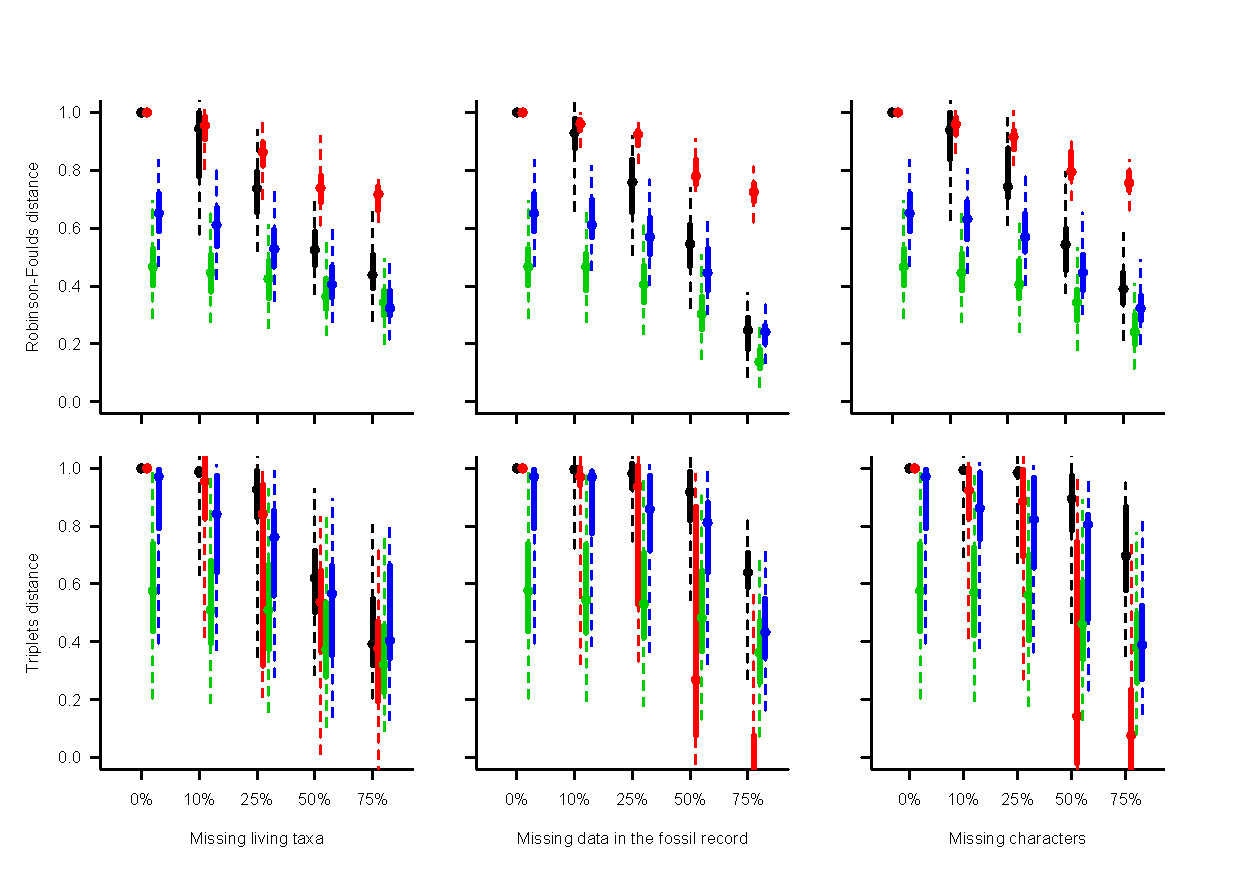
\includegraphics[width=1\textwidth]{Figures/In_main/AllMethods-RF+Tr-colour.pdf}
\caption{The effects of increasing missing data on topological recovery using Maximum Likelihood trees (black), Bayesian consensus trees (red), Maximum Likelihood bootstrap trees (green) and Bayesian posterior tree distributions (blue). The percentage of missing data for each parameter ($M_{L}$, $M_{F}$ and $M_{C}$) is shown on the x axis. Topological recovery was measured using two different tree comparison metrics: Normalised Robinson-Foulds distance (upper row) and Normalised Triplets distance (lower row). The graph shows the modal value (points), the 50\% (thick solid lines) and 95\% (thin dashed lines) confidence intervals of the distributions of the tree comparison metric for each missing data parameter and tree inference method. }
\label{Fig_Results-permeth_perparam} %Differences within a subset of parameters and between methods
\end{figure}

% NC: Y axes should be standardised Robinson Foulds
% NC: X-axes should have (Mc) etc in brackets after the names
% NC: Also should probably have the X axes read : Missing character (Mc, %) and remove % from tick labels
% TG: Ok, will fix later on since it's all scripted (no illustrator cheats)

%NC: I would rewrite these figure labels as follows. I prefer the details of colours and things to be in brackets not in the text. Rewrite the others in a similar fashion.
%NC: Remeber it's not topology, but topological recovery that you are measuring
%The effects of increasing missing data on topological recovery using Maximum Likelihood trees (black), Bayesian consensus trees (red), Maximum Likelihood bootstrap trees (green) and Bayesian posterior tree distributions (blue). The percentage of missing data for each parameter ($M_{L}$, $M_{F}$ and $M_{C}$) is shown on the x axis. Topological recovery was measured using two different tree comparison metrics: Normalised Robinson-Foulds distance (upper row) and Normalised Triplets distance (lower row). The graph shows the modal value (points), the 50\% (thick solid lines) and 95\% (thin dashed lines) confidence intervals of the distributions of the tree comparison metric for each missing data parameter and tree inference method. 

\begin{figure} 
\centering
    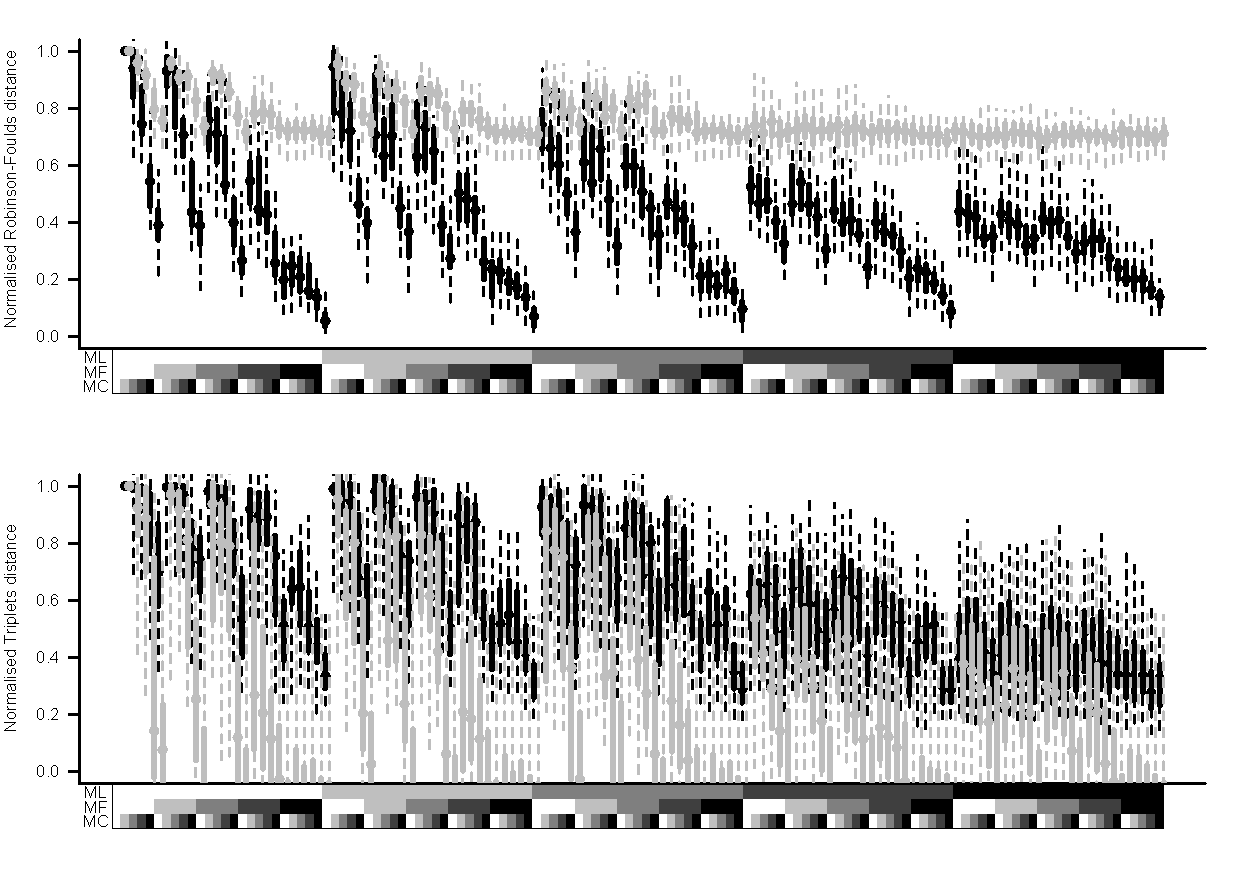
\includegraphics[width=1\textwidth]{Figures/In_main/ML+Baycon-AllParam-RF+Tr-BW.pdf}
\caption{Effect of increasing missing data on topological recovery using Maximum Likelihood trees (black) and Bayesian consensus trees (grey). The percentage of missing data (gradient colour from 0\% (white), 10\%, 25\%, 50\% and 75\% (black)) for each parameter ($M_{L}$ (upper line), $M_{F}$ (middle line) and $M_{C}$(lower line)) is shown on the x axis. Topological recovery was measured using two different tree comparison metrics: Normalised Robinson-Foulds distance (upper row) and Normalised Triplets distance (lower row). The graph shows the modal value (points), the 50\% (thick solid lines) and 95\% (thin dashed lines) confidence intervals of the distributions of the tree comparison metric for each missing data parameter and tree inference method.} 
\label{Fig_Results-global_perparam} %Differences between all the parameters and between two methods (ML vs BC)
\end{figure}

%Hide this figure for 'fast' build
%\begin{figure} 
%\centering
%    \includegraphics[width=1\textwidth]{Figures/In_main/PairwiseComp-Baycon-RF+Tr-colour.pdf}
%\caption{Effect of missing data on topological recovery using Bayesian consensus trees. The percentage of missing data (gradient colour from 0\% (white), 10\%, 25\%, 50\% and 75\% (black)) for each parameter ($M_{L}$ (upper line), $M_{F}$ (middle line) and $M_{C}$(lower line)) is shown on both x and y axis. Topological recovery is represented by the probability of the two different tree comparison metrics (Normalised Robinson-Foulds distance (A - right) and Normalised Triplets distance (B - left)) distribution overlap with the "best" tree using the the Bhattacharyya Coefficients (low probability of overlap - red ; high probability of overlap - green).}
\label{Fig_Results-paircomp_within}
%\end{figure} %Pairwise BC for the Bayesian consensus trees for RF and TR. (parameters differences)

%Removed figure (table instead)
%\begin{figure} 
%\centering
  %  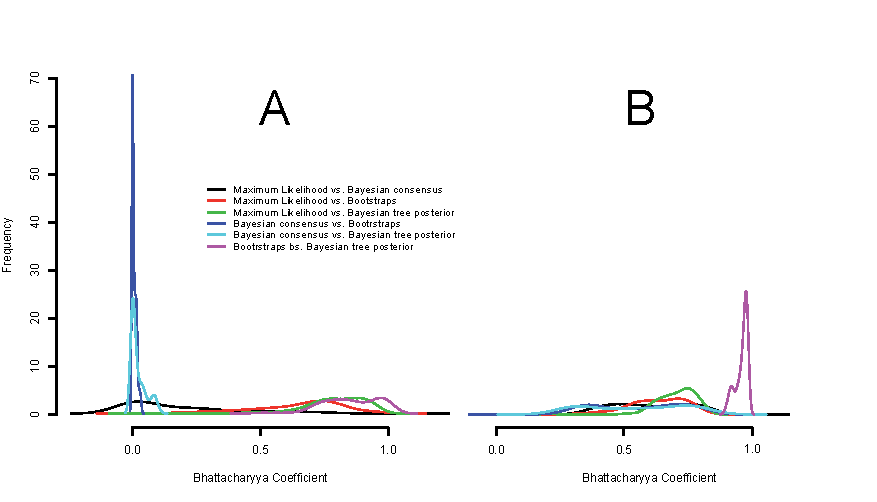
\includegraphics[width=1\textwidth]{Figures/In_main/BC-MethodComp-RF+Tr-colour.pdf}
%\caption{Distribution of the Bhattacharyya Coefficients between methods. Curves represents the kernel density estimations of the Bhattacharyya Coefficients between the four different methods. A. Results for the Normalised Robinson-Foulds distance. B. Results with the for Normalised Triplets distance. Pikes around the two different extremes values of the Bhattacharyya Coefficients show the two pairs of most dissimilar methods (Bayesian consensus vs. Bootstraps and Bayesian consensus vs. Bayesian posterior trees) for the Normalised Robinson-Foulds distance ; and the most similar methods (Bootstraps and Bayesian posterior trees) for the Normalised Triples methods.}
%\label{Fig_Results-paircomp_without} %Comparisons between methods, both in RF and Triplets.(method differences)
%\end{figure}

% TG: Put this table in landscape!
\begin{table}[ht]
\caption{Bhattacharyya Coefficients of the pairwise method comparisons, each of which corresponds to the normalised distance between the "best" tree and the "missing data".}
\centering
\begin{tabular}{lccccccc}
  \hline
 Comparison &  Metric & Min. & 1st Qu. & Median & Mean & 3rd Qu. & Max. \\ 
  \hline
    Maximum Likelihood \textit{vs.} & $RF^1$ & 0.00 & 0.00 & 0.10 & 0.20 & 0.32 & 1.00 \\ 
    Bayesian consensus              & $Tr^2$ & 0.34 & 0.49 & 0.61 & 0.62 & 0.75 & 1.00 \\ 
    Maximum Likelihood \textit{vs.} & $RF^1$ & 0.03 & 0.54 & 0.69 & 0.64 & 0.77 & 0.98 \\ 
    Maximum Likelihood bootstraps   & $Tr^2$ & 0.08 & 0.57 & 0.65 & 0.64 & 0.73 & 0.82 \\ 
    Maximum Likelihood \textit{vs.} & $RF^1$ & 0.02 & 0.74 & 0.80 & 0.79 & 0.89 & 0.98 \\ 
    Bayesian posterior trees        & $Tr^2$ & 0.21 & 0.67 & 0.73 & 0.72 & 0.77 & 0.84 \\ 
    Bayesian consensus \textit{vs.} & $RF^1$ & 0.00 & 0.00 & \textbf{0.00} & \textbf{0.01} & 0.01 & 0.04 \\ 
    Maximum Likelihood bootstraps   & $Tr^2$ & 0.08 & 0.38 & 0.59 & 0.57 & 0.73 & 0.84 \\ 
    Bayesian consensus \textit{vs.} & $RF^1$ & 0.00 & 0.00 & \textbf{0.01} & \textbf{0.02} & 0.04 & 0.11 \\ 
    Bayesian posterior trees        & $Tr^2$ & 0.21 & 0.36 & 0.56 & 0.55 & 0.74 & 0.87 \\ 
    Bayesian posterior tree \textit{vs.}  & $RF^1$ & 0.50 & 0.77 & \textbf{0.85} & \textbf{0.85} & 0.96 & 1.00 \\ 
    Maximum Likelihood bootstraps   & $Tr^2$ & 0.91 & 0.96 & \textbf{0.98} & \textbf{0.97} & 0.99 & 1.00 \\ 
   \hline
\end{tabular}
   $^1RF$=Normalised Robison-Fould distance ; $^2Tr$=Normalised Triplets distance
\label{Tab_Results-Difference_methods}
\end{table}


%Bleuah! Changing everything to stick to 5 parts as
%Part 1: missing data decrease topology
%Part 2: effect of ML
%   -As missing data increase, topology decreases
%   -This is different for the metrics
%   -This is worst with that method
%       (e.g. Distribution of RF values for the ML difference % missing data a substantial overlap with bla (BC=88, Fig bla))
%Part 3: effect of MF 
%Part 4: effect of MC
%Part 5: combined effect

%Part 1
As the amount of missing data in the morphological part of the total evidence matrix increases, our ability to recover the "best" tree's topology decreases, regardless of the missing data parameter ($M_{L}$, $M_{F}$ or $M_{C}$), the method of tree inference (Maximum Likelihood or Bayesian) or the tree comparison metric used (Normalised Robinson-Foulds or Normalised Triplets distance). However, the different missing data parameters and tree inference methods do not affect the topology in the same way (Fig.~\ref{Fig_Results-permeth_perparam} and Fig.~\ref{Fig_Results-global_perparam}). In any combination of parameters or metrics, the Maximum Likelihood bootstraps trees and the Bayesian posterior distribution trees performs in a substantially similarly (Table ~\ref{Tab_Results-Difference_methods}) and worth than the Maximum Likelihood and the Bayesian consensus trees (Fig.~\ref{Fig_Results-permeth_perparam} - see discussion). %add discussion link

%Part 2
\subsection{Individual effects of missing data parameters} 
As the amount of missing data increases across all three parameters, the ability to recover the "best" tree's topology decreases (Fig.~\ref{Fig_Results-permeth_perparam}). However, the decrease of the Normalised Robinson-Fould distance plateaus at minimum of 0.69 for Bayesian consensus tree (Fig.~\ref{Fig_Results-permeth_perparam} and Fig.~\ref{Fig_Results-global_perparam} - see also \hyperref[SupplementaryMaterial]{Supplementary Material Section 3} for the table of values) and there is no substantial difference in topological recovery for 50\% or 75\% of missing living taxa (upper triangle in Fig.~\ref{Fig_Results-paircomp_within}-A). Therefore, clades seems to be more conserved in the Bayesian consensus tree more than any other method (see discussion).  %add discussion link
On the other hand, the decrease in Normalised Triplets distance is less contrasted with a greater overlap of Normalised Triplets distance with the Maximum Likelihood tree (Fig.~\ref{Fig_Results-permeth_perparam}) - mean Bhattacharrya Coefficient=0.10 for the Normalised Robinson-Foulds distance and 0.61 for the Normalised Triplets distance - see table ~\ref{Tab_Results-Difference_methods}).

%Part 3
\subsection{Effect of missing data for fossil taxa ($M_{F}$)}
As the amount of missing data in the fossil part of the matrix increases, the ability to recover the "best" tree's topology decreases as well (Fig.~\ref{Fig_Results-permeth_perparam}). For the Robinson-Fould distance, we observe the same pattern than for $M_{L}$ with a better topological recovery of the Bayesian consensus trees on any other methods (Fig.~\ref{Fig_Results-permeth_perparam} and Fig.~\ref{Fig_Results-global_perparam}). However, the Normalised Triplets distance drops drastically when going from 25\% of missing data to 50\% (mode) %get the modal values here
making this parameter more sensible to wildcard taxa in the Bayesian consensus tree (Fig.~\ref{Fig_Results-permeth_perparam} - see discussion). %add discussion link

%Part 4
\subsection{Effect of missing character ($M_{C}$)}
As described for the two previous parameters $M_{L}$ and $M_{F}$, an increase in the amount of missing characters decreases the ability to recover the "best" tree's topology decreases (Fig.~\ref{Fig_Results-permeth_perparam}). Similarly again, the Bayesian consensus trees shows higher Normalised Robinson-Fould distance than the Maximum Likelihood tree (Fig.~\ref{Fig_Results-permeth_perparam}). And in a similar way as for the $M_{F}$ parameter, the Normalised Triplet distance drops drastically when going from 25\% of missing data to 50\% (mode). %get the modal values here

%Part 5
\subsection{Combined effect of missing data parameters ($M_{L}$, $M_{F}$ and $M_{C}$)} 
The combine of the missing data parameters ($M_{L}$, $M_{F}$ and $M_{C}$) reduces the ability to recover the "best" tree's topology when each parameters contains a maximum of missing data (i.e. $M_{L}$=75\%, $M_{F}$=75\% and $M_{C}$=75\% - Fig.~\ref{Fig_Results-global_perparam} and see \hyperref[SupplementaryMaterial]{Supplementary Material Section 3} for the combined effects of the parameters in both Normalised Robinson-Foulds and Normalised Triplets distance for the Maximum Likelihood Bootstraps trees and the Bayesian posterior trees distribution). Regarding the clade conservation (i.e. the Normalised Robinson-Foulds distances), the Bayesian consensus tree greatly outperforms the Maximum likelihood trees with Normalised Robinson-Foulds scores always superior than 0.69 (Fig.~\ref{Fig_Results-global_perparam} - see also \hyperref[SupplementaryMaterial]{Supplementary Material Section 3} for the exact values) regardless the combination of missing data parameters (Fig.~\ref{Fig_Results-paircomp_within}-A). However, for the Normalised Triplets distance, the Bayesian consensus tree often displays negative values (i.e. differences greater than expected by chance) but with few substantial differences (Fig.~\ref{Fig_Results-paircomp_within}-B). Also the differences between the Normalised scores of the Maximum Likelihood trees and Bayesian consensus trees are substantially difference for the Normalised Robinson-Foulds distance (mean Bhattacharrya Coefficient=0.10) and for the Normalised Triplets distance (mean Bhattacharrya Coefficient=0.61 - see table ~\ref{Tab_Results-Difference_methods}). Thus the sensitivity of the Bayesian consensus trees to wild card taxa is not highly different than the one for the Maximum likelihood trees (i.e. the distribution of Normalised Triplets distance have a high probability of overlap). The results of the probability of overlap between the pairwise distributions of Normalised Robinson-Foulds and Triplets distances of the Maximum Likelihood trees, the Maximum Likelihood Bootstrap trees and the Bayesian posterior trees distribution is available in the \hyperref[SupplementaryMaterial]{Supplementary Material Section 3}.


%Binned removed bits from former results.

%As the amount of missing data in the morphological part of the total evidence matrix increases, our ability to recover the "best" tree's topology decreases, regardless of the missing data parameter ($M_{L}$, $M_{F}$ or $M_{C}$), the method of tree inference (Maximum Likelihood or Bayesian) or the tree comparison metric used (Normalised Robinson-Foulds or Normalised Triplets distance). 
%However, the different missing data parameters and tree inference methods do not affect the topology in the same way (Fig.~\ref{Fig_Results-permeth_perparam} and Fig.~\ref{Fig_Results-global_perparam}). % And figure 3 too right? TG: Yep
%The Normalised Robinson-Foulds distance calculate for the trees inferred in Maximum Likelihood framework decreases with the increase of missing data in our three parameters ($M_{L}$, $M_{F}$ or $M_{C}$) with a modal Normalised Robinson-Fould score always below 0.5 when 75\% of the living taxa have no data ($M_{L}$=75\% - Fig.~\ref{Fig_Results-global_perparam}). However, in Bayesian inference, the ability of the method (the Bayesian consensus tree) to recover a "best" tree's topology plateaus at a minimal Normalised Robinson-Fould score of 0.69 (Fig.~\ref{Fig_Results-global_perparam} - see \hyperref[SupplementaryMaterial]{Supplementary Material Section 3} for the values distribution). The results of the topological recovery with the parameters combination in both Normalised Robinson-Foulds and Triplets distances for the Maximum Likelihood bootstrap trees and the Bayesian posterior distribution trees are available in the \hyperref[SupplementaryMaterial]{Supplementary Material Section 3}.
%All parameters combinations are different than the "best" tree (always red) in both metrics.
%The lowest probability of overlap (low Bhattacharrya Coefficient values) between pairwise distributions of parameters combinations ($M_{L}$, $M_{F}$ and $M_{C}$ with 0\%, 10\%, 25\%, 50\% or 75\% missing data) is always between the comparison of Normalised distance (Robinson-Foulds or Triplets) of the "missing data" tree with no missing data ($M_{L}$=0\%, $M_{F}$=0\% and $M_{C}$=0\%) and all the other "missing data" trees.
%The parameters combinations are less dissimilar in Triplets than in RF (less red).
%However, pairwise comparisons are more dissimilar (low Bhattacharrya Coefficient values) in the Normalised Robinson-Fould distance results than in the Normalised Triplets distance results.
%The ML parameter (0% and 10%) are more different in RF and Triplets (red stripes at the base). The ML parameter (50, 75) are the more similar (green upper part) in RF.
%The Normalised Robinson-Fould distance for the comparisons between the trees with a low amount of missing data for the living taxa ($M_{L}$=0\% and 10\%) shows the most dissimilarities with the other parameter combinations.
%The combination of the ML parameter (0% and 10%) and the MC parameter (0, 10, 25) are the most different (details on the red stripes).
%Check supplementary for the rest
%The results of the probability of overlap between the pairwise distributions of Normalised Robinson-Foulds and Triplets distances of the Maximum Likelihood trees, the Maximum Likelihood Bootstrap trees and the Bayesian posterior trees distribution is available in the \hyperref[SupplementaryMaterial]{Supplementary Material Section 3}.
%When looking at the pairwise Bhattacharyya Coefficients between all the parameters combinations for Bayesian consensus trees, % NC: Instead just state the result. "We found that number of missing living taxa ($M_{L}$) results the lowest probabilities of overlap (table X)". In the same way as you wouldn't say "Using a linear regression we found that x ~ Y." You'd say "X and Y were significantly correlated (Table1)".
%NC: Also what IS the result really? You find that ML overlaps less with the other parameters so it's significantly different in it's effect? And from the graph you can see it's worse? What does oerlap MEAN in terms of the answer to the question, i.e. how do the parameters affect topological recovery. 
%the number of missing living taxa ($M_{L}$) results the lowest probabilities of overlap (right lower corner in Fig.~\ref{Fig_Results-paircomp_within}-A). However, when looking at the Triplets distance, because of the high overlap in confidence intervals, there is no major region with low probability of overlap. One should note however that the bottom line of the matrix where the Bhattacharyya Coefficients are very low is due to comparing the distribution of the pairwise comparison of the "best" tree against the "missing-data" tree with no missing data ($M_{L}$=0\%, $M_{C}$=0\%, $M_{F}$=0\%) , leading to a normalised Triplets score of 1 every time (with no variance, see Fig.~\ref{Fig_Results-permeth_perparam} and Fig.~\ref{Fig_Results-global_perparam}). The pairwise comparisons for the other methods (Maximum Likelihood, Bootstraps and Bayesian posterior trees) are available in the supplementary materials (see \hyperref[SupplementaryMaterial]{Supplementary Material Section 3}).
%NC: I'd start by describing the pattern with reference to figs 2 and 3 and then the "significant" results
%When looking at the comparisons between the methods 
%using the Robinson-Foulds distance, the Bayesian consensus trees have the least overlap with respectively the Bayesian posterior trees and the Bootstrap (Fig.~\ref{Fig_Results-paircomp_without}-A). Using the Triplets distance, the two methods that have the most distribution %NC: ???
%are the Bootstraps and the Bayesian posterior trees (Fig.~\ref{Fig_Results-paircomp_without}-B). These results are due to the difference in comparing topologies between Maximum Likelihood and Bayesian consensus trees and Bootstraps and Bayesian posterior trees: the latter two are based on a random pairwise comparison of a sub-sample of 1000 trees. This is likely to add noise to the data.


%---------------------------------------------
%
%       DISCUSSION
%
%---------------------------------------------

% NC: Quick comment. You find that Bayesian consensus trees are "best". BUT I think you need to be careful here with what you mean by "best". They are most likely to recover a more similar topology to the best tree than if you do the crazy tree comparison pairs. But that doesn't mean they're best, just that they perform best in your simulations. They are only best for that. If you want to advise people to use a method that best recovers topology as measured using RF or Triplets, then Bayesian consensus is best. BUT generally that is not what people want. Probably need to think some more about this.
% TG: a note about the "best" tree's topology regarding your comment just after the discussion header: should I replace "correct" by "best" since that's how we're calling the "best" tree anyway (all in quotes)


\section{Discussion}

Our results show that the ability to recover the "best" tree's topology in a Total Evidence framework decreases with increasing missing data, regardless of how data were removed or the method of tree inference used. However, these factors affected topological recovery in different ways and to different extents. 
Decreasing the overall number of morphological characters in the matrix ($M_{C}$) and the amount of living taxa with morphological data ($M_{L}$) had worst effects on topological recovery (Fig.~\ref{Fig_Results-paircomp_within}). Additionally, using Bayesian consensus trees recovered the "best" tree's topology more consistently than using Maximum Likelihood trees or Bayesian posterior trees distributions (Fig.~\ref{Fig_Results-global_perparam} and Fig.~\ref{Fig_Results-paircomp_within}).
% ----->
% NC: Probably needs another summing up line here. Or maybe not
% <-----
% NC: Make sure it's parameters then tree building methods. NC: Make sure the order of the parameters is always the same L,F, C or whatever! THROUGHOUT the paper. Also correct RF and T to standardised OR normalised RF and T.
% NC: Might want to add a couple of subheadings to match those in the results.
As proposed in previous studies, our results show that the amount of missing data is not a problem \textit{per se} for Total Evidence methods, as long as enough morphological characters overlaps for most taxa in the matrix \citep[e.g.][]{kearneyfragmentary2002,wiensmissing2003,rouresite-specific2011,pattinsonphylogeny2014}. % NC: What do you mean by data overlap here? That species have overlapping characters?

\subsection{Effect of missing living taxa ($M_{L}$)} %Or remove? Also below then
%What is the parameter variation doing in our simulation
When the number of living taxa with morphological data ($M_{L}$) decreases, entire rows of data are being removed from the living taxa part of the matrix. Because living taxa still have 10 times more molecular characters available, even if they have no morphological data, the relation between them will always be fairly well resolved (depending on the phylogenetic signal from the molecular part of the matrix) and thus, ignoring the fossils, the living taxa clades will be always well conserved. However, this missing data parameter influences a lot the placement of fossil taxa because a decrease of the $M_{L}$ parameter will reduce the overlapping data between the living and the fossil taxa.

%Methods
%Part saying the difference between ML and Baycon
When using the Normalised Robinson-Foulds distance to measure topological similarity, the Bayesian consensus trees recover the "best" tree's topology more often than Maximum Likelihood trees (Fig.~\ref{Fig_Results-global_perparam}). In fact, regardless of the amount of missing data, Bayesian consensus trees always displays the highest Normalised Robinson-Foulds score (always $>$ 0.69; see \hyperref[SupplementaryMaterial]{Supplementary Material Section 3} for details). However, regarding the Normalised Triplets distance, the topological similarity with the "best" tree's topology decreases in the same way for both the Maximum Likelihood trees and the Bayesian consensus trees (Fig.~\ref{Fig_Results-permeth_perparam} and Fig.~\ref{Fig_Results-global_perparam}).
%Part saying the difference between BS and baytrees
Regardless of the metric, the Maximum Likelihood boostrap trees and the Bayesian posterior trees distribution always performed poorlier in their ability to recover the "best" tree's topology, even when no morphological data was missing ($M_{L}$=0\% - Fig.~\ref{Fig_Results-permeth_perparam}). This reflects the fact it is difficult to compare two distributions of trees, and each comparison between a set of "missing data" tree and "best" tree in these cases involved 1000 random pairwise comparisons rather than just one. This will obviously add noise to the results for these two methods.

%Metrics
%Part explaining the differences between the metrics
This difference between the metrics is linked to what they measure and how they perform at doing it (see method %add link
, \hyperref[SupplementaryMaterial]{Supplementary Material S2} and \citealt{kuhnerpractical2014} for details on the nature of both metrics). In the Bayesian consensus tree topology, the clade conservation (i.e. Noramlised Robinson-Foulds distance) stays always high but the placement of wildcard taxa (i.e. the Normalised Triplets distance) decreases way faster (Fig.~\ref{Fig_Results-permeth_perparam} and Fig.~\ref{Fig_Results-global_perparam}). This is due to the fact that both metrics are illustrating two different aspects of tree topology (i.e. clade conservation for the Normalised Robinson-Foulds distance and wildcard taxa position for the Normalised Triplets distance - see method %add link!
and \hyperref[SupplementaryMaterial]{Supplementary Material S2} for details on both metrics). However, it is important to note that The Normalised Robinson-Foulds distance is more sensitive than the Normalised Triplets distance: when getting closer to the root of the tree, displacement of single taxon makes the clades not being exactly identical any more even if the clade still contains all the other taxa in both trees. Also, \citet{kuhnerpractical2014} have recently demonstrated that the Robinson-Foulds distance outperforms the Triplets distance for measuring topological differences between trees. Thus, the Bayesian consensus tree's topology seems to be the less affected by removing morphological data for living taxa (Fig.~\ref{Fig_Results-permeth_perparam} and Fig.~\ref{Fig_Results-global_perparam}).

\subsection{Effect of missing data for fossil taxa ($M_{F}$)}
%When the overall proportion of data for the fossil taxa ($M_{F}$) decreases, this reduces the probability of morphological characters for the fossil taxa to overlap with the ones for the living taxa and leads to displacement of certain taxa. However, it is important to note that even though the number of displaced wildcard taxa increases (i.e. decrease of Normalised Triplets distance), the conservation of the clades (i.e. Normalised Robinson-Foulds distance) is still relatively good (mode=% value
%) when the proportion of missing data is high ($M_{F}$=75\%).

%Methods
%Decrease in clade conservation is smaller than for param ML in the Bayesian consensus tree for the clade conservation but higher than param ML for the displacement of wildcard taxa. This is due to the fact that the Bayesian consensus tree is a majority consensus rule and that when the fossils have less data, they kind of randomly branch all over the shop and therefore no majority consensus position (>50\% of the time) exists puting the fossil on a politomie at the base of a clade (clade conservation stays high but displacement of taxa increases). On the opposite in MaxLik, the topology is always dichotomous but the fossil can be missplaced in the wrong clade (with a low BS value) but is moving less. In other words, Bayesian consensus tree places the fossil with a higher confidence at a low taxonomic level (politomy) and the MaxLik places the fossil with a low confidence at a high taxomomic level (baldy supported dichotomies). We can argue that the first option (higher confidence at a low taxonomic level) is preferable (example the Darwinius debate).

\subsection{Effect of missing character ($M_{C}$)}
%When the overall number of morphological characters in the matrix ($M_{C}$) decreases

%Story for MC: MC is expected to have an effect two times bigger than ML or MF, e.g. removing 10\% of MF removes 5\% of data (because it works only on the fossil part) and removing 10\% of MC actually removes 10\% of that.
%Method
%However the effect of removing characters has an effect of topology of the same order of magnitude than for ML and MF (FigRes 1): For RF, Bayesian consensus is better than ML and for Tr, MaxLik is better than Baycon and have the same drop at 50\% as for MF (different than for ML). 

%In this scenario, the overall number of missing characters ($M_{C}$) affects the proportion of overlapping data by reducing the overall size of the matrix (Fig.~\ref{Fig_Results-global_perparam}). % NC: What's the relevance of that sentence?
%However, the pairwise Bhattacharyya Coefficients show that the area with the lowest probability of distributional overlap is led by comparing the trees with no missing data for the living taxa to the trees with 75\% missing data for the living data (right lower corner in Fig.~\ref{Fig_Results-paircomp_within}). %NC: I don't understand what you mean here

\subsection{Combined effect of missing data parameters ($M_{L}$, $M_{F}$ and $M_{C}$)} 
%In our simulations, the overlap in data is greatly reduced when all three missing data parameters have a lot of missing data (e.g. $M_{L}$ = 75\%, $M_{F}$ = 75\% and $M_{C}$ = 75\%; Fig.~\ref{Fig_Results-permeth_perparam} and Fig.~\ref{Fig_Results-global_perparam}).
%When combining the effect, we 

%Our solutions
Our missing data parameters illustrate different sources of missing data in empirical matrices as follows: ($M_{L}$) the paucity of coded morphological characters for living taxa; ($M_{F}$) missing data for fossils (or parts of fossils) that have not been preserved in the fossil record; and ($M_{C}$) characters that have not been coded across living and fossil species, perhaps due to difficulties in coding or poor preservation of the feature in collections. Filling these gaps in empirical Total Evidence matrices should lead to a substantial increase in our ability to recover the "best" tree's topology. We can increase the number of living taxa with coded morphological characters by increasing research efforts in this area, and encouraging use of our vast natural history collections. Increasing data for fossil species is harder, since it depends on fossil preservation biases and new fossil discoveries. However, gaps in the matrix can be filled with future discoveries of exceptionally preserved fossils \citep[e.g.][]{nithe2013}. Fortunately, although this data is the most difficult to collect, it also has the least influence on whether our simulations recover the "best" tree's topology (Fig.~\ref{Fig_Results-paircomp_within}). Finally, although increasing the number of coded characters is relatively straightforward, the amount of time it takes to build a morphological matrix increases directly with the number of characters involved. One solution to this problem may be to engage with collaborative data collection projects through web portals such as \textit{morphobank} \citep{morphobank}, so that no one individual collects all the data.


% ----->
% TG: Put that part somewhere in the start with the discussion of ML vs Baycon in the effect of ML part?
%-Probabilistic method always better (wright but see spencer) - Check McGuire[nope]/Sean[nope] literature for Bayesian vs. ML?
Variation in our ability to recover the "best" tree's topology also depended heavily on the method used to infer the tree (Fig.~\ref{Fig_Results-permeth_perparam} and Fig.~\ref{Fig_Results-global_perparam}). Previous studies have shown some superiority of methods using simple probabilistic models such as the M\textit{k} model \citep{lewisa2001} over cladistic methods (\citealt{wrightbayesian2014}; but see \citealt{spencerefficacy2013}). However, this is the first study, to our knowledge, that compares the performance of the M\textit{k} model \citep{lewisa2001} using Maximum Likelihood and Bayesian methods in a Total Evidence framework. %TG: I guess it's a good selling point: we ARE the first ones to do a sensitivity analysis in a TEM framework (as far as I know).
% <-----

%Discussing results 2
%   -Why is Baycon so different than Baytre? Since Baycon is calculated from Baytre.
Also, in the case of the lower performances of the Bayesian consensus trees when using the Triplets distance, one can note the high overlap of the confidence intervals (Fig. ~\ref{Fig_Results-permeth_perparam} and Fig. ~\ref{Fig_Results-paircomp_within}-B). % NC: Don't get the relevance of the last sentence/why it fits here. Can you expand?
% NC: Probably want some  statement here about bayesian being better than ML, and if you want to fix a single topology in TE we recommend a bayesian consensus. If you want to account for tree uncertainty we recommend a bayesian posterior distribution. Our results dont suggest this is bad, but more suggest that we can't compare trees very well in this case.

% $§4: Thus, baycon seems the best way to go >...
% ^§5: >... but we have to take into account problems in our protocol.

%\label{metrics_discussion}
%This difference between the metrics can be explained by their respective ability to measure the differences between two trees \citep{kuhnerpractical2014}. As shown in Fig.~\ref{Fig_Results-permeth_perparam} and Fig.~\ref{Fig_Results-global_perparam}, the contrast between the results of the two metrics can be explained by the actual nature of both metrics (see \hyperref[SupplementaryMaterial]{Supplementary Material S2}):
%\begin{enumerate}
%\item{The Robinson-Foulds metric is a conservative metric, which is more sensible to single taxon displacement because it will count clades as similar only if they are composed of the same taxa with the same topologies \citep{RF1981}. When getting closer to the root of the tree, displacement of single taxon makes the clades not being exactly identical any more even if the clade still contains all the other taxa in both trees. This metric illustrates therefore the conservation of clades among the compared trees (i.e. when the normalised Robinson-Foulds distance is close to 1, most of the clades in the two trees are identical).}
%\item{On the other hand, the Triplets method is measuring the position of each taxon towards two other reference taxa \citep{critchlowthe1996}. It will penalise only trees when taxa get removed furthest from their original position. This metric therefore illustrates the amount of wildcard taxa \citep{kearneyfragmentary2002} between the two compared trees (i.e. when the score is closed to 1, few wildcard taxa are present in the tree).}
%\end{enumerate}
%Therefore, in our study, both metrics are showing two different aspects of tree topology. For example, regarding the Bayesian consensus trees, completes clade are conserved most of the time (Fig.~\ref{Fig_Results-global_perparam}-top) but with an increasing amount of missing data, wildcard taxa get more and more displaced (Fig.~\ref{Fig_Results-global_perparam}-bottom). Because we are comparing the Baysian consensus tree to a single tree topology, the probability of recovering the exact position of a wildcard taxa than in the "best" tree is really low and even reducing with the amount of missing data. Regarding this fundamental differences, the Robinson-Foulds metric performs better in showing a distance from the true topology than the Triplets distance \citep{kuhnerpractical2014}. Therefore, the results for the Bayesian consensus trees can be preferred on the Maximum Likelihood trees because - when using the Robinson-Fould distance - they display a higher ability to recover the "best" tree's topology (Fig. ~\ref{Fig_Results-permeth_perparam}).




%Opening/further work part - NC(meeting): Be less defensive (i.e. nothing seemed to have gone wrong THIS time).
%   -Simulating morpho characters
The variations in our results could also be explained by another methodological caveat: 
% NC: What variations do you mean? Only an issue if it might bias results in one direction or another
the performance of our simulation protocol. In order to reduce the computational time of our analysis ($~$150 CPU years), we ran our sensitivity analysis on modestly sized matrices of 1000 molecular characters and 100 morphological characters. These matrices are two orders of magnitude smaller than some matrices used in published analyses \citep[e.g.][]{springermacroevolutionary2012,nithe2013} but still ranges in the sizes of smaller matrices used in other ones \citep[e.g.][]{sallam2011craniodental,kellymolecular2014}. %TG: note about NOT citing O'Leary here. 1-I don't like the paper ; 2-the Ni et al paper (primates) as a big morpho matrix too (1k  characters against 4k for O'Leary, same order of magnitude?) ; 3-We might want to limit the papers we're citing? note about citing Sean's and your paper here: 1-is it okay (regarding last time warning of being extra careful when citing you're own work)?
Also, simulating morphological characters is more complex than molecular ones. The underlying pattern of their evolution is often more complex and ruled by more parameters than molecular characters (i.e the number of character states, the states frequencies, the substitution matrix and the statistical model used) \citep{Pagel22011994,wagner2000,lewisa2001,wrightbayesian2014}. Morphological characters studies involve many potential statistical pitfalls (e.g. independent characters violation, rate variation - \citet{davalosintegrating2014}) and especially (i) incongruence with molecular signal and (ii) homoplasy \citep{wagner2000}.
\begin{enumerate}
\item{First, morphological data can display a different signal than molecular data, especially in small matrices \citep{wagner2000}. %REF
This might lead to a controversial phylogenetic signal in the overall matrix and lower down the support values. However, regarding empirical data studies, most of the groups shows fairly congruent morphological and molecular phylogenetic signal \citep[e.g.][]{leerates2013}.}
\item{Secondly, in this study, we made the assumption that theoretically, morphological characters are randomly distributed on an organism however it seems clear that empirical morphological data does not act randomly \citep{sansomfossilization2013,pattinsonphylogeny2014}. However, following our simulation assumption of random character distributions, if they accumulate through time in the same way as the majority of the molecular characters then, homoplasic characters are expected to appear randomly through time \citep{davalosintegrating2014}. Therefore, homoplasy is expected to be more important (by chance) in bigger morphological matrices \citep{davalosintegrating2014}. After reaching a critical amount of morphological characters, adding new ones increases homoplasy \citep{wagner2000}.}
\end{enumerate}

% $§6: Knowing the caveats, we can try to fix them >...
% ^§7: >... by taking into account data realness (fossil templates and rate heterogeneity).

%§7
%Further directions - is that necessary though?
% NC: Cut for now, might want to put these ideas in the appropriate places above instead.
%   -Using real data
%One way to address this issue 
% NC: Which issue???
%would be to run a similar analysis using real data. The amount of studies using Total Evidence data type matrices is steadily increasing \citep[e.g.][]{ronquista2012,slaterphylogenetic2013,beckancient2014} and one could analysis these total evidence matrices in the same framework as this study. However, the true topology (obtained from a matrix with no missing data) is unlikely to be known. A second way to address this issue, and especially to incorporate the variation of signal in morphological character would be to simulate morphological characters at different rates \citep{wrightbayesian2014} or to apply patterns of missing data directly obtained from the fossil record \citep{pattinsonphylogeny2014}. Nevertheless, our simulation already show clear results of the effect of missing data on topology in a Total Evidence framework. Also, our results show how recovering the "best" tree's topology can be improved by using Bayesian consensus trees in combination with a maximum amount of characters and a of living taxa with morphological data.
%   -Looking at branch length?

% $§7: But despite the caveats above, missing data is not a big deal >...
% ^§8: >... We can use TEM for integrating fossils into trees.

%§8
%Back to the importance of TEM - How we can use fossils (Intro-§2)
%   -Data is not a major problem
%Despite the various caveats discussed above, we answered our main question on how does Total Evidence matrices perform in recovering topology with different methods and different amounts of missing data.
% NC: For a concluding paragraph, don't start by reminding people of the caveats! End strongly and confidently
% Also no need to restate the question - instead give the answer.
%   -Good and promising method.
%Our results shows that this method performance decreases mainly with a reduction in the overlap of morphological data. To address this problem, we propose to increase the data overlap by coding living species and to have a large morphological matrix. Also, our results shows disparity among methods and a clear superiority %NC: Not really 
%of the Bayesian consensus tree topology over the Maximum Likelihood one.

%---------------------------------------------
%
%       CONCLUSION
%
%---------------------------------------------

\section{Conclusion}

%§Conclusions
% part 1- Fossils are important and can be used combined with living taxa (Intro-§1 & §2)
%   -TEM works with missing data
% part 2- This is how we can improve the data to use them in the best way possible (Conclusion-§1 & §8)
%   -Use bayesian consensus
%   -Go code living taxa
Using Total Evidence matrices with missing data is not a problem for recovering the "best" tree's topology as long as enough morphological data is overlapping between the fossil and living taxa. %NC: Explain more clearly what you mean by overlap - of characters?
Topological recovery is still best when there is less missing data, therefore we advise filling as many gaps in Total Evidence matrices as possible. Because this is difficult, if not impossible, for fossil data, we recommend coding as many


using as many morphological characters as possible and to code them for a maximum of living taxa present in the matrix.


we propose to use the Bayesian consensus tree over the Maximum Likelihood tree or over a random subset of the Bayesian posterior trees distribution. Also, in order to improve the overlap in data in the morphological part of the matrix, 

% NC: Never write "in order to". Just "to" will do

%---------------------------------------------
%
%       ...
%
%---------------------------------------------
\section{Supplementary material}
Supplementary material (R code, analyses, supplementary methods and full results) can be found in the Dryad data repository at http://dx.doi.org/10.5061/dryad.XXXX. %section and sentence format asked by Syst. Biol.

\section{Acknowledgements}
Thanks to Fr\'{e}d\'{e}ric Delsuc, Emmanuel Douzery, Andrew Jackson, Gavin Thomas and April Wright. %TG : Not sure how many people we have to thank but it could also include Graham Slater, Nick Matzke and Trevor Hodkinson.
 % NC: Might be nice to thank Trevor, and it won't add too many lines to thank them all. You can also just calle people A.Wright if you want to reduce word count.
for useful comments on our simulation protocol.
%Thanks to Sive Finlay, Kevin Healy and Adam Kane for comments on the manuscript. %TG: or helping writing sentences does not really count. % NC: Depends how much they helped. I just used to thank the lab for that stuff
Thanks to Paddy Doyle, Graziano D'Innocenzo and Sean McGrath for assistance with the computer cluster. Simulations used the Lonsdale cluster maintained by the Trinity Centre for High Performance Computing and funded through grants from Science Foundation Ireland. This work was funded by a European Commission CORDIS Seventh Framework Programme (FP7) Marie Curie CIG grant (proposal number: 321696).

%cite cheat sheet
 % The \cite command functions as follows:
 %   \citet{key} ==>>                Jones et al. (1990)
 %   \citet*{key} ==>>               Jones, Baker, and Smith (1990)
 %   \citep{key} ==>>                (Jones et al., 1990)
 %   \citep*{key} ==>>               (Jones, Baker, and Smith, 1990)
 %   \citep[chap. 2]{key} ==>>       (Jones et al., 1990, chap. 2)
 %   \citep[e.g.][]{key} ==>>        (e.g. Jones et al., 1990)
 %   \citep[e.g.][p. 32]{key} ==>>   (e.g. Jones et al., p. 32)
 %   \citeauthor{key} ==>>           Jones et al.
 %   \citeauthor*{key} ==>>          Jones, Baker, and Smith
 %   \citeyear{key} ==>>             1990

\bibliographystyle{sysbio}
\bibliography{References}
%Needs to be cleaned a bit
% NC: Yeah. Leave it til we send it to Gavin but it should be a priority. Almost all of them are wrong! 
%---------------------------------------------
%
%       Supplementary, separated
%
%---------------------------------------------

%Ignore this for 'fast' pdf building
%\section{Supplementary Material}

%    \section{Code}
All code for performing the analyses is available at: \url{https://github.com/TGuillerme/Total\_Evidence\_Method-Missing\_data/tree/master/Functions} The tree comparison analysis can be repeated using code available at: \url{https://github.com/TGuillerme/Total\_Evidence\_Method-Missing\_data/tree/master/Analysis} %fully running! Try it at home (5-10 minutes of data loading)!

\newpage
\section{Supplementary Material 1: Tree Building}
  %\section{Supplementary material 1 : Tree building}

\subsection{Morphological character states}
To obtain a realistic value for the probability of having \textit{k} characters states for each simulated morphological character, we randomly selected 100 morphological matrices, each with more than 100 characters each, from TreeBASE (http://treebase.org/). We only selected matrices published between 1985 and 2013 and covering 19 taxonomic classes (Chordata, Arthropoda, Annelida, Angiosperm, Gymnosperm and Pteridophyta). This resulted in a total of 22563 characters that had between two and 10 character states. We then extracted the proportion of characters with each number of states (two to 10) to give us an empirical estimate of the average number of character states for each character, as shown in Figure \ref{Fig_AppendixCharacters}. Most characters have two or three states, therefore we only simulate characters with two or three states, and sample these in proportion to their occurrence in our empirical data ()% NC: Can we put the probabilities here, I know they are in the main text)

%We then sampled 22563 \textit{k} values between two and 10 with the same proportion of characters from the empirical data. We then used a simple t-test to check if our simulation was equal to the empirical data.
% NC: I don't know why this t-test or these simulations were run...

%In this study, we only simulated characters with 2 or 3 states because of the high proportion of ordered characters encountered on characters with more than 3 states and the difficulties of simulate biologicaly sensible ordered characters.

\begin{figure}
\centering
\includegraphics[keepaspectratio=true]{Figures/Supplementary/TEM_Fig-AppendixCharacters.pdf}
\caption{The proportion of morphological characters with between two and 10 character states extracted from 100 randomly selected empirical matrices downloaded from TreeBASE.}
\label{Fig_AppendixCharacters}
\end{figure}
% NC: Can you remove the title of this figure?

\newpage
\subsection{Tree Building Software settings}

For clarity we have provided the exact settings used in our tree building below.

\subsubsection{Maximum Likelihood: RAxML version 8.0.20 \citep{Stamatakis21012014}}

\begin{itemize}
  \item Molecular data: GTR + $\Gamma_4$ (-m GTRGAMMA)
  \item Morphological data: Mk + $\Gamma_4$ (-K MK)
  \item Support: Rapid Boostrap algorithm (LSR), 1000 replicates
\end{itemize}

\subsubsection{Bayesian: MrBayes version 3.2.1 \citep{Ronquist2012mrbayes}}

\begin{itemize}
  \item Priors
  \begin{itemize}
    \item Molecular data
    \item Rates distribution shape ($\alpha$) = 0.5
    \item Transition/Transversion ratio = 2 ($\beta$(80,40))
    \item Starting tree: "True" tree topology with each branch length = 1
  \end{itemize}
  \item Morphological data
  \begin{itemize}
    \item rates distribution shape ($\alpha$) = 0.5
  \end{itemize}
  \item Models
  \begin{itemize}
    \item Molecular data: HKY + $\Gamma_4$
    \item Morphological data: Mk + $\Gamma_4$
  \end{itemize}
  \item MCMC
  \begin{itemize}
    \item Two runs
    \item Four chains per run
    \item Generations < 50$\times$$1^6$
    \item Sample frequency = 1050$\times$$1^3$
    \item ASDS diagnosis frequency = 50$\times$$1^3$
    \item ASDS $<$ 0.01
    \item ESS $>>$ 200
    \item Burnin = 25\%
  \end{itemize}
\end{itemize}
  \label{Supp_TreeBuilding}

\newpage
\section{Supplementary Material 2: Tree Comparisons}
  \subsection{Triplets metric details ($T_{x,y}$)}
Each triplet can be written as $I_{ijk}$=(\textit{ijk})). Where $I_{ijk}$ is equal to 0 if the the two triplets (\textit{ijk}) are the same in the two trees otherwise $I_{ijk}$ is equal to 1.
For any rooted tree there are only four possible combinations per triplets: ((\textit{j},\textit{k}),\textit{i});, ((\textit{i},\textit{k}),\textit{j}); and ((\textit{i},\textit{j}),\textit{k}); and (\textit{i},\textit{j},\textit{k}); \citep{johnson1998}.
One can calculate $S_n$, the triplet distance between two trees as:
\begin{equation}
S_n = \sum_{ijk} I_{ijk}
\end{equation}
Where:
\begin{equation}
\sum_{ijk} = \binom{n}{4} = \frac{n!}{4!(n-4)!}
\end{equation}
And where n is the number of taxa in both trees (modified from \citet{critchlowthe1996}).
When all triplets across the two trees are the same, $S_n$ is equal to 0 and when all the triplets are different $S_n$ is equal to $\binom{n}{4}$.
Because the possible number of triplets per clade is a finite number, the probability of two random trees with the same n taxa to have the same triplet is:
\begin{equation}
P({I_{ijk}}=0) = \frac{1}{4}
\end{equation}
Therefore one can calculate the probability of two random trees having the same triplets: 
\begin{equation}
P({S_{n}}=0) = \sum_{ijk} P_{I_{ijk}=0}
\end{equation}
\begin{equation}
P({S_{n}}=0) = \frac{n!}{4(3!(n-3)!}
\end{equation}
And in the same way:
\begin{equation}
P({S_{n}}=1) = \frac{3n!}{4(3!(n-3)!}
\end{equation}

\subsection{RF metric details}
The RF distance (or path difference) between two trees reflects the distance between the distributions of the tips among clades in the two trees \citep{RF1981} and can be expressed as following:
\begin{equation}
RF_{x,y} = N_{x} + N_{y} - 2C_{x,y}
\end{equation}
Where $C_{x,y}$ is the number of clades in common in the two trees. 
The minimal value of \textit{C} is equal to 1 if the two trees have the same n taxa;
the maximal value in \textit{C}=\textit{n}-2.
For a fully unresolved tree (star tree) \textit{N}=1 and for a fully resolved tree (binary tree) \textit{N}=\textit{n}-2.
The minimal and maximal topological distance for \textit{n} taxa is:
\begin{equation}
RF_{min} = 1 + 1 - 2C_{x,y}
\end{equation}
And:
\begin{equation}
RF_{max} = 2(n-2)-2
\end{equation}
One can then rescale \textit{RF.scaled} by using the maximal and minimal value for any \textit{n} taxa:
\begin{equation}
RF.scaled_{x,y} = \frac{RF_{x,y}-RF_{max}}{RF_{max}}
\end{equation}
This metric is more sensitive to taxa displacement than the Triplet distance \citep{critchlowthe1996,johnson1998,wiensmissing2003} and therefore a low value will show a good clade conservation between two trees and a high value will show a bad recovery of common clades.

\subsection{Tree comparisons}
\subsubsection{Random tree comparison scaling}
We used the comparison of 1000 random trees to obtain the mean comparison value $\bar{d}_{m,n}$\textit{(rand)} for the NTS metric.
We randomly generated two sets of 1000 trees of \textit{n} taxa using the rmtree function of ape package (v3.0-11 \citet{paradisape:2004}) that generates a given number of random Yule trees.
We calculated the $\bar{d}_{m,n}$\textit{(rand)} value using an approach similar to the RPCBTC (described below) by performing 1000 random pairwise comparisons using the TreeCmp java script \citep{Bogdanowicz2012}.

\subsubsection{Random Pairwise Bayesian Tree Comparison (RPBTC)}
We assessed the power of the Random Pairwise Bayesian Tree Comparison (RPBTC) method by comparing 1000 random trees from a posterior distribution trees set to another 1000 random trees from the same posterior distribution trees set.
We repeated this 100 times independently using the same posterior distribution trees set each time resulting in 100 replicates of the same posterior distribution trees set compared 1000 times.
We used an ANOVA to test if there was no significant difference between the replicates so that the RBTC can be replicated.
We applied this protocol on a poorly resolved tree (Low Score), a resolved tree with low support value (Medium Score) and a resolved tree with high support values (High Score).
Results are available in table ~\ref{RPBTC_testing}. %link broken

\begin{table}[ht]
  \caption{Group comparison results: difference between 100 replicates using the RPBTC method} %test with TreeCmp.anova
  \centering
  \begin{tabular}{rllrrrr}
  \hline
  Tree.Type & Used.metric & Replicates & Df & F.value & p.value \\ 
  \hline
  Low Score & RF & 100.00 & 99.00 & 0.74 & 0.98 \\ 
  Low Score & Tr & 100.00 & 99.00 & 0.97 & 0.58 \\ 
  Medium Score & RF & 100.00 & 99.00 & 0.64 & 1.00 \\ 
  Medium Score & Tr & 100.00 & 99.00 & 0.45 & 1.00 \\ 
  High Score & RF & 100.00 & 99.00 & 0.20 & 1.00 \\ 
  High Score & Tr & 100.00 & 99.00 & 0.37 & 1.00 \\ 
  \hline
\end{tabular}
  \label{RPBTC_testing}
\end{table}

  \label{Supp_TreeComparison}

\newpage
\section{Supplementary Material 3: Additional Results}
  \section{Supplementary material Section 3}

\begin{figure} 
\centering
    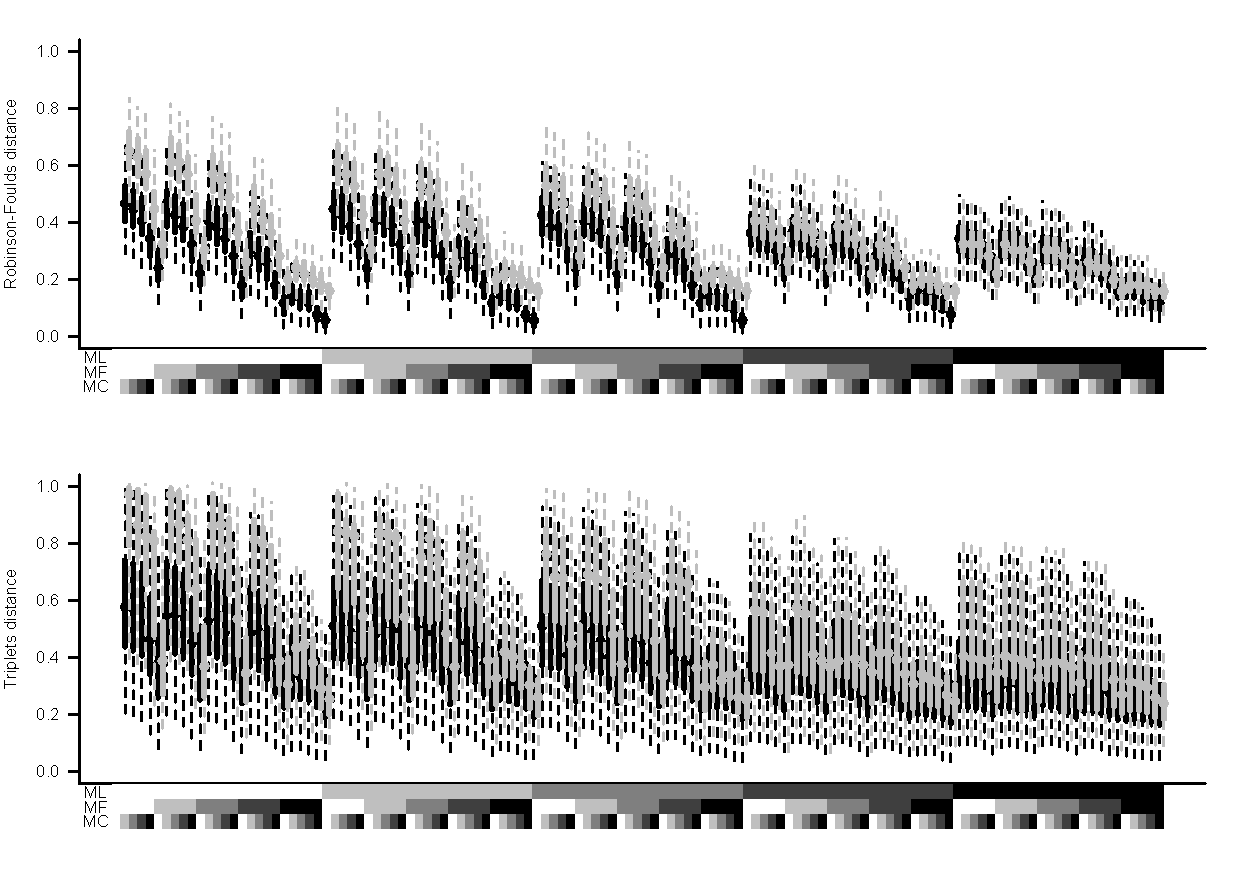
\includegraphics[width=1\textwidth]{SupplementaryMaterial/Supp_Figures/Boot+Baytre-AllParam-RF+Tr.pdf}
\caption{Trend of the effect of missing data on topological recovery on the Bootstraps and the Bayesian posterior trees distributions. The amount of missing data per parameter ($M_{L}$, $M_{F}$ and $M_{C}$) is represented along the x axis. The colour gradient from white to black represents respectively, 0\%, 10\%, 25\%, 50\% and 75\% of missing data. The topological recovery is represented on the y axis, both using Robinson-Foulds distance (upper row) and Triplets distance (lower row). Points represent the modal value of each distribution ; thick solid and thin dashed lines represents respectively the 50\% and 95\% confidence intervals or the distributions. The Bootstraps are represented in black and the Bayesian posterior trees distributions in grey.}
\label{Fig_global_BootTreesets} %Differences between all the parameters and between two methods (Boot vs treesets)
\end{figure}

\begin{figure} 
\centering
    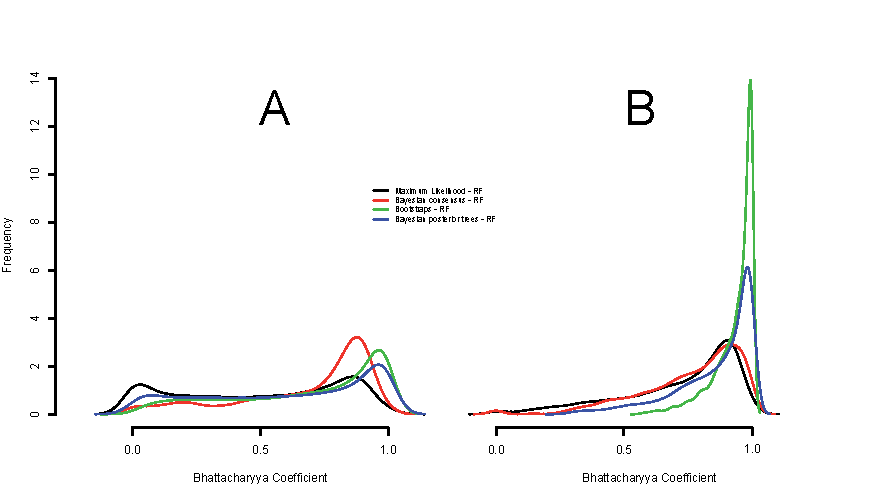
\includegraphics[width=1\textwidth]{SupplementaryMaterial/Supp_Figures/BC-AllMethods-RF+Tr.pdf}
\caption{Distribution of the Pairwise Bhattacharyya Coefficients within each method. A- Distribution of the coefficients when comparing Ronbinson-Foulds distances. B- Distribution of the coefficients when comparing Triplets distances.}
\label{Fig_Bhatt.coeff_distribution} %Differences in overlap within each method
\end{figure}

\begin{figure} 
\centering
    \includegraphics[width=1\textwidth]{SupplementaryMaterial/Supp_Figures/PairwiseComp-ML-RF+Tr.pdf}
\caption{Pairwise Bhattacharyya Coefficients within the Maximum Likelihood trees. The pairwise trees comparisons are represent on both axis. The colour gradient from white to black represents respectively, 0\%, 10\%, 25\%, 50\% and 75\% of missing data for each parameter. The matrix represents the values of pairwise Bhattacharyya Coefficients going from green (1) to red (0). A. Results for the Normalised Robinson-Foulds distance. B. Results with the for Normalised Triplets distance.}
\label{Fig_pairComp-Baytree-RF}
\end{figure} %Pairwise BC for the ML for RF+Tr. (parameters differences)

\begin{figure} 
\centering
    \includegraphics[width=1\textwidth]{SupplementaryMaterial/Supp_Figures/PairwiseComp-Boot-RF+Tr.pdf}
\caption{Pairwise Bhattacharyya Coefficients within the Bootstrap trees. The pairwise trees comparisons are represent on both axis. The colour gradient from white to black represents respectively, 0\%, 10\%, 25\%, 50\% and 75\% of missing data for each parameter. The matrix represents the values of pairwise Bhattacharyya Coefficients going from green (1) to red (0). A. Results for the Normalised Robinson-Foulds distance. B. Results with the for Normalised Triplets distance.}
\label{Fig_pairComp-Baytree-Tr}
\end{figure} %Pairwise BC for the Boot for RF+Tr. (parameters differences)

\begin{figure} 
\centering
    \includegraphics[width=1\textwidth]{SupplementaryMaterial/Supp_Figures/PairwiseComp-Baytre-RF+Tr.pdf}
\caption{Pairwise Bhattacharyya Coefficients within the Bayesian posterior distribution trees. The pairwise trees comparisons are represent on both axis. The colour gradient from white to black represents respectively, 0\%, 10\%, 25\%, 50\% and 75\% of missing data for each parameter. The matrix represents the values of pairwise Bhattacharyya Coefficients going from green (1) to red (0). A. Results for the Normalised Robinson-Foulds distance. B. Results with the for Normalised Triplets distance.}
\label{Fig_pairComp-MLbest-RF}
\end{figure} %Pairwise BC for the Baytre for RF+Tr. (parameters differences)


\begin{table}[ht]
\centering
\begin{tabular}{rrrrrrr}
  \hline
 & Min. & 1st Qu. & Median & Mean & 3rd Qu. & Max. \\ 
  \hline
  Maximum likelihood-RF & 0.06 & 0.26 & 0.40 & 0.41 & 0.50 & 0.95 \\ 
  Maximumlikelihood-Tr & 0.29 & 0.45 & 0.59 & 0.63 & 0.84 & 1.00 \\ 
  Bayesian consensus-RF & 0.69 & 0.71 & 0.72 & 0.76 & 0.79 & 0.96 \\ 
  Bayesian consensus-Tr & -0.28 & -0.11 & 0.17 & 0.19 & 0.37 & 0.98 \\ 
  Bootstraps-RF & 0.06 & 0.18 & 0.27 & 0.26 & 0.34 & 0.46 \\ 
  Bootstraps-Tr & 0.23 & 0.31 & 0.35 & 0.38 & 0.45 & 0.58 \\ 
  Bayesian posterior trees-RF & 0.16 & 0.22 & 0.32 & 0.34 & 0.42 & 0.65 \\ 
  Bayesian posterior trees-Tr & 0.24 & 0.35 & 0.40 & 0.50 & 0.67 & 0.98 \\ 
   \hline
   \hline
\end{tabular}
\end{table}
  \label{Supp_results}
%    \label{SupplementaryMaterial}

%END
\end{document}